+% 
% This is Jody Grady's Thesis
%

% This starts the document; the "npsreport" style is really a modified
% report style. Feel free to use the options:
%
% "twoside" - prints "THIS PAGE INTENTIONALLY LEFT BLANK" on
%             odd-numbered pages at the end of sections.
%
% "traditional" - prints a ``traditional'' NPS thesis style, rather
% than the new one.
% See also /opt/local/share/texmf-dist/tex/latex/base/report.cls

%\documentclass[twoside,traditional]{npsreport} 
%\documentclass[twoside]{npsreport} 
%\documentclass[twoside,authorindex,thesis]{npsreport} 
\documentclass[twoside,thesis]{npsreport} 
\securitybanner{}
\usepackage{pdfpages}
\usepackage{amsmath}
\usepackage{supertabular}
\usepackage{longtable}
\usepackage{tabularx}
\usepackage{multicol}
\usepackage{eufrak}
%\usepackage{ulem}
\usepackage{setspace}
\usepackage{hyphenat}
\usepackage{listings}
\usepackage{xcolor}
\usepackage[pdftex,
  pdftitle={\@title}, 
  pdfauthor={\@author},
  pdfkeywords={parts based object detection, computer forensics},
  pdfpagemode=UseOutlines,
  bookmarks,
  bookmarksopen=false
  citecolor=black,
  filecolor=black,
  linkcolor=black,
  urlcolor=black,
  urlbordercolor=white,
  linkbordercolor=white,
  citebordercolor=white,
  filebordercolor=white,
  menubordercolor=white,
  runbordercolor=white,
  pdfstartview={XYZ null null 1.22}]{hyperref}

% Here are some commands that will help you make more attractive LaTeX
%
% Reference commands
%
% And here is the main thesis

\urlstyle{rm}
\title{Author Attribution on a Mobile Phone}
\author{Jody Grady}
\rank{Commander, United States Navy}
\degree{Master of Science in Computer Science}
\department{Department of Computer Science}
\thesisadvisor{Robert Beverly}
\secondreader{Craig Martell}
\departmentchair{Peter J. Denning}
\prevdegrees{B.E. Georgia Institute of Technology, 1994}
\degreedate{March 2011} 
\distribution{Approved for public release; distribution is unlimited}
\RPTpreparedFor{}
\abstract{ Put something abstracty here.....}

% Information for the SF298.
% These are mandatory:
\ReportType{Master's Thesis}
\DatesCovered{2009-03-01---2011-03-25}
\SponsoringAgency{National Reconnaissance Office}
\ReportClassification{Unclassified}
\AbstractClassification{Unclassified}
\PageClassification{Unclassified}

\SupplementaryNotes{ The views expressed in this thesis are those of
  the author and do not reflect the official policy or position of the
  Department of Defense or the U.S. Government. \textbf{\footnotesize
    IRB Protocol Number: n/a}}

% These are optional:
\ContractNumber{}
\GrantNumber{}
\ProgramElementNumber{}
\TaskNumber{}
\WorkUnitNumber{}
\POReportNumber{}
\Acronyms{}
\SMReportNumber{}


\SubjectTerms{Machine Learning,Author Attribution,Mobile Computing, Supervised Learning}
\ResponsiblePerson{}
\RPTelephone{}
% Set up the floats properly. I love my floats!
\setcounter{topnumber}{10}   % up to 10 floats at the top of the page; Should be enough
\setcounter{totalnumber}{10} % see above
%
% your thesis begins here
%
% This must be on a line by itself:

\begin{document}

\NPScover                       % Cover
\NPSsftne                       % SF298
\NPSthesistitle                 % Title page
\NPSabstractpage                % Abstract Page
\NPSfrontmatter                 % NPS front matter follows

% This changes the chaptermark and includes the various tables

\renewcommand{\chaptermark}[1]{\markboth{\MakeUppercase{\chaptername}\ \thechapter.\ #1}{}}
\tableofcontents\cleardoublepage
\listoffigures\cleardoublepage
\listoftables\cleardoublepage

% I put the acknowledgements here
\acknowledgements{
..... I would like to thank all the little transistors that computed the results I got here....
}

% NPS body follows

\NPSbody
\include{rules}


\chapter{Introduction}
 % Introduction
\chapter {Prior and Related Work}

\section {Introduction}
Detecting authors on mobile devices requires selection of a feature set that distinguishes authors, selection of techniques that effectively uses these features to identify authors, selection of efficient machine learning

\section {Author Detection}
"Automated authorship attribution is the problem of identifying the author of an anonymous text, or text whose authorship is in doubt" \cite{love_attributing_2002}.  For this thesis, author detection and authorship attribution are synonymous.  The explosive growth of communications and document storage on the Internet provides a vast amount of data to draw on for author detection.  Books, articles, blogs, tweets, and emails are posted for public viewing in an electronic format every day.  Some of these postings have verifiable authors.  Many Internet authors use nom de plumes or are posted anonymously.  The increased speed and storage capacity of computing devices allow analysis of these corpora for author detection.

\section {Machine Learning}
"Machine learning is programming computers to optimize a performance criterion using example data or past experience" \cite{alpaydin_introduction_2004}.  Machine learning has been used famously to determine the authors of the Federalist papers, allow computers to "read" human handwriting, and to mine sales data for profitable trends.  Two broad categories of machine learning are supervised learning and unsupervised learning.  Supervised learning is "learning with a teacher."  The teacher can show the learner what to do based on examples or experience. Unsupervised learning is "learning with a critic" \cite{alpaydin_introduction_2004}. This thesis relies exclusively on supervised learning because identifying authors on mobile devices requires construction of an author model away from the mobile device.  That model is then put on a device for ongoing author identification.  The models require previous "teaching" instead of predictive "criticizing".

Machine learning is comprised of a set of classes, a classifier, a feature set, and data.  In supervised learning, the machine learner uses a data input comprised of features fitted to (or owned by) by a specific class.  Based on creatively counting these features, the machine learner creates a model for each class based on the the behavior of the classifier.  Finally, test data, consisting of sets of features, are processed by the classifier based on the previously built models.  The classifier provides an output of the most likely class that fits the given features.

Machine learning is central to this thesis.  Modeling corpora of emails and tweets from numerous authors on large computers, and, then, testing prediction capability on mobile devices requires not just accurate machine learning, but efficient machine learning.  The efficiency is needed due to the limits of even the most advanced mobile devices.

	\subsection {Machine Learning Techniques}
	The techniques in this thesis are all supervised.  Specifically, the two supervised techniques used are Naive Bayes and Support Vector Machine (SVM).  Naive Bayes was chosen because it is computationally lightweight compared to many other methods.  Support Vector Machine was chosen because data for SVM can be stored in "sparse format".  Sparse means that every feature does not have to be represented in the stored data for a model or test case.  Features with a zero count can simply be excluded.  SVM has been successful in many other authorship attribution experiments \cite{jurafsky_speech_2009}.

		\subsubsection{Naive Bayes}
			\paragraph{} Naive Bayes is a supervised learning method that uses Bayes Rule of probability chaining over a set of features (words in a document) to arrive at an overall probability that a specific a set of features (words in a document) belongs to a particular class (specific author). Naive Bayes uses a strong independence assumption among the various features.  This means that the classifier assumes that the probability of one feature appearing in a data set is completely independent of another feature showing up in the data set.  While this independence of features is unlikely to be actually true, the independence keep the calculation of probabilities simple.  In the case of documents and authors, Naive Bayes represents a bag of words model of a document where word order is lost and only frequency or occurrence of words or word combination is captured. The probability that a document, d, belongs to a given class, c, is given by:
				\begin{equation} P(c|d) \propto P(c) \prod_{i<k<n_d} P(t_k|c) \end{equation}

			\paragraph{} To specifically apply the above equation to author detection, the classifier returns the class with the highest probability after executing the above formula.  This turns the above equation into a maximum a posteriori (MAP) class $c_{map}$:
				\begin{equation} c_{map} = arg \: max \; \hat{P}(c|d) = arg \: max \; [ \hat{P}(c) \prod_{i<k<n_d} \hat{P}(t_k|c) ] \end{equation}

			since underflow is an issue when numerous float values are multiplied together over a set of features, the practical application of the above formula is:
				\begin{equation} c_{map} = arg \: max \; \hat{P}(c|d) = arg \: max [ log \: \hat{P}(c) + \sum_{i<k<n_d} log \: \hat{P}(t_k|c) ] \end{equation}

			??? My code does not have a prior -- am I messing this up?  The project in machine learning did not have a given prior either, investigate this!!! ???
			
			Since the probability of each feature is multiplied by the probability of every other feature, a zero probability for any feature will make the overall probability zero.  To handle this issue, smoothing is used.  Smoothing is a method of adding some non-zero values to each feature to prevent zero values.  The simplest form of smoothing is Laplace (Plus One Smoothing).  In this method, each feature in the feature set is initialized with a count of 1 instead of zero.  The denominator in the probability equation is increased by $1 * number of features$ to account for all the added ones.  This method often produces undesirable results.  For this thesis, the counts from words in the Google Web1T corpus are used to smooth word counts in Naive Bayes.  The specific details of the Google Web1T corpus are covered in a later section of this chapter.

		\subsubsection{Support Vector Machine}
		A Support Vector Machine (SVM) is a supervised learning method that find a separating line or shape through a set of data based on a feature set.  This is based on finding a boundary between two types of data in a dataset, then computing the largest boundary between closest data points and the boundary.  In cases where a clear boundary between two data sets is not possible, a "slack variable" provides an allowance of data points to be on the wrong side of the boundary. To create the boundary, SVM "maps the input vectors into some high dimensional feature space, Z, through some non-linear mapping chosen a priori" \cite{vapnik_support-vector_1995}

		Two situations: 1) data can be separated without error and 2) data cannot be separated without error.

			\paragraph{Historical Roots of Support Vector Machines}
			SVM historical roots lie in the R.A. Fischer's pattern recognition work using a Variance/Covariance matrix \cite{fisher_use_1936}.  Fisher's pattern recognition used the mean matrix (also know as the centroid of a matrix) and  variance-covariance matrix (also known as the dispersion of a matrix) of two normal distributions, and found the optimal Bayesian solution was a non-linear function.  Fisher simplified his non-linear function to a linear function for situations where the dispersion of both normal distributions are equal.  He even found that his simplified linear equation worked satisfactorily when the distributions needing patterns recognized were not strictly normal.

				%\begin{equation}\label{Variance} \frac{(\mathbf{x} -\mathbf{m} ) (\mathbf{x} - \mathbf{m})}{n} \end{equation}

				%\begin{equation}\label{Covariance} \frac{(\mathbf{x} - \mathbf{m}) (\mathbf{y} - \mathbf{m)}}{n} \end{equation} 

			From this basis, Fisher created a precedent of pattern recognition based on linear discriminating surfaces within a multi-dimensional space.  Fisher's work was furthered by perceptron work in the 1960's.  This work created multiple linear discriminating surfaces to find a matching pattern.  However, there was no method to optimize the separation between data using perceptrons.  From the need to optimize the separation, feedback mechanisms were developed to refine the perceptron weights. By further developing the idea of feeding back to the perceptron weights, SVMs were created.

			\paragraph{SVM Base Equations}
				\subparagraph {Probability of Error} E being expectation value of the probability of committing an error on a test example is bounded by the ration between the expectation value of the number of support vectors and the number of training vectors:

				\begin{equation} E[Pr(error)] \leq \frac{E(number\ of\ support\ vectors)}{number\ of\ training\ vectors}\end{equation}

				\subparagraph{Optimal Hyperplane in Feature Space}
				\begin{equation}\label{oh1} \mathbf{w_0} \cdot \mathbf{z} + b_0 = 0\end{equation} where $w_0$ are weights, $z$ is the space, and $b_0$ is still a mystery to me.
				To that end, $\mathbf{w_0}$ "can be written as some linear combination of support vectors."  This uses the following equation:
				\begin{equation}\mathbf{w_0} = \sum_{support\ vectors} \alpha_i \mathbf{z_i}\end{equation} and the decision function using those weights is given by
				\begin{equation}I(z) = sign\left(\sum_{support\ vectors} \alpha_i \mathbf{z_i} \cdot \mathbf{z} + b_0\right)\end{equation}

				\subparagraph*{Optimal Hyperplanes}
				For distance $\rho$ between projections defined by the support vectors, $\rho$ is defined as:
				\begin{equation}\rho(\mathbf{w}, b) = \min_{x:y=1} \frac{\mathbf{x} \cdot \mathbf{w}}{ |\mathbf{w}|} - \max_{x:y=-1} \frac{\mathbf{x} \cdot \mathbf{w}}{|\mathbf{w}|}\end{equation}
				given that \eqref{oh1} it follows that the weights needed to create the optimal hyperplane are given by
				\begin{equation}\label{oh2} \rho (\mathbf{w_0}, b_0) = \frac{2}{|\mathbf{w_0}|}\end{equation}  The best solution maximizes the distance $\rho$.  To maximize $\rho$, you must minimize the magnitude of $\mathbf{w_0}$.  Find that minimum $\mathbf{w_0}$ is a quadratic programming issue.

				\subparagraph{Procedure} "Divide the training data into a number of portions with a reasonable small number of training vectors in each portion.  Start out by solving the quadratic programming problem determined by the first portion of training data.  For this problem there are two possible outcomes: either this portion of the data cannot be separated by a hyperplane (in which case the full set of data as well cannot be separated), or the optimal hyperplane for separating the first portion of the training data is found." If this first set is found to be linearly separable, then all the non-support vector values are discarded, a new batch of values are put into this set (these values do not meet the constraint of $y_i(\mathbf{w} \cdot \mathbf{x_i} + b) \ge 1, i = 1,...,{l}$ )
				\subparagraph*{Soft Margins}
				In cases where the data is not linearly separable, the goal becomes to minimize the number of errors (the number of values on the wrong side of the hyperplane).  Now a new variable $\xi \ge 0, i=1,...,l$ is introduced along with the function $\Phi (\xi) = \sum_{i=1}^{l} \xi_{i}^{\sigma}$ .  The constraints are that the value 
				$\xi_i$ does not push values in the non-negative quadrant out of the negative quadrant ( $y_i(\mathbf{w} \cdot \mathbf{x_i} + b) \ge 1 - \xi_i, i=1,...,l$.  Also, $\xi_i$ is zero or a positive number ( $\xi_i \ge 0$).  $\xi$ here represents "the sum of deviations of training errors"
				The central equation for minimizing the number of errors is:
				\begin{equation}\label{soft_margin}  \frac{1}{2}\mathbf{w^2} + CF(\sum_{i=1}^{l} \xi_{i}^\sigma)\end{equation}
				In cases for $ \xi_{i}^{\sigma} $ where $\sigma=1$, we are dealing with the soft margin hyperplane.  Cases where $\sigma < 1$, there may not be a unique solution.  For values of $\sigma > 1$, there are also unique solutions, but $\sigma =1$ is the smallest value and that allows the term $CF(\sum_{i=1}^{l} \xi_{i}^\sigma)$ from \eqref{soft_margin} to not overwhelm  the $frac{1}{2}\mathbf{w}^2$.
			\paragraph{Multi-Class SVM}



	\subsection {Machine Learning Tools}

		\subsubsection{LibSVM} LibSVM attempts to optimize the SVM equation 
		\begin{equation} \min_{\mathbf{w}, b, \xi} \frac{1}{2} \mathbf{w^t w} + C \sum_{i=1}^{l} \xi_i \end{equation}
		\begin{equation} \text{subject to } y_i( \mathbf{w^t}\phi ( \mathbf{x}_i ) + b ) > 1- \xi_i \end{equation}
		\begin{equation} \text{and } \xi_i > 0.

		For all kernels used in SVM a variable that must be solved for prior to optimization, the penalty term, $C$.  Other kernels have additional variables that must be solved for prior to optimization, such as \gamma in the RBF kernel.  While there are sophisticated methods to find C and other required variables, LibSVM takes a simple, straighforward approach: grid search.  The grid for this search is a log grid search.  As the local minimum is found on each pass of the grid search, libSVM reduces the grid size to home in on the minimum C value.  

			\paragraph{} To make libSVM more efficient and more likely to converge on a solution, data in the training set should be scale to either span 0 to +1 or -1 to +1.  While test data may show up outside the original training data range, libSVM will extend the normalized range to accomodate.  For example, if the range of the training data was -100 to +100, libSVM would scale that range to -1 to +1.  If there was test datum with a value of -110, then libSVM would scale that datum to -1.1.  While it is stated here that libSVM scales data, that function is not automatic within libSVM itself, but is rather part of the libSVM.
		
			\paragraph{} LibSVM was originally constructed in C (VERIFY) and employed with python tools to support.  LibSVM is not available in a wide array of languages, including Java.  A Java version of libSVM makes libSVM functional on many of the mobile operating systems available today, including Android.  For this reason, libSVM was originally chosen as the SVM tool for this thesis.


		\subsubsection{LibLinear}  While libSVM has numerous kernel to improve results, the inclusion of code to accomdate these kernels slows libSVM down.  To increase processing speed for libSVM for linear kernels, libLinear was created.  LibLinear removes all code in libSVM except for code explicitly used for a linear kernel.  A linear kernel has been found to give as good or nearly as good a result as other kernels such as RBF, parabolic, and radial for text classification, especially when the corpus being used is large.  The reduction is code can produce resutls 100-200 times faster that using LibSVM.

			\paragraph{} LibLinear has also been studied for large data sets that produces models which cannot be fit into memory.
			

\section {Features}

	\subsection {Feature Types}

	\subsubsection {N-Grams}

	\subsubsection{Gappy Bigrams}

	\subsubsection{Orthogonal Sparse Bigrams}

	\subsection {Feature References} Feature selection is the process of deciding which features to include during classification. A set of features can be built from the training set, such as selecting N most used words in a training set.  Features can be further refined by using outside references.  For instance, a feature set could be built as the N most used words in a training set and filtered for stop words.  In this case, stop words could be defined by other researchers work or some standard stop word set.  Another option is to build all features from a reference set.  This thesis made heavy use of the Google Web1T Corpus to act as a feature filter and a feature reference.

	\subsubsection{Google Web1T Corpus} 
		\paragraph{} The Google Web1T Corpus is a massive corpus of English language N-grams ranging from N=1 to N=5.  The corpus was created from a snapshot of Google's search databases that took place during January 2006.  The corpus consists of text files with the N-grams accompanied by a count of those N-grams.  Each set of N-grams is stored in its own folder.  The N-Grams are organized alphabetically by the first word in the N-Gram.  For instance, "a cat" comes before "a dog" in the 2-Grams of the corpus.  The unique folder within the corpus is the 1-Gram folder.  There are two files within the 1-Gram folder.  One file is organized alphabetically like the rest of the corpus, but the other file is organize by count.  The largest count comes first.
		\paragraph{} Punctuation is included in the corpus.  Sentence boundaries are indicated by $<$S$>$ and $<\backslash\text{S}>$.  To qualify for corpus inclusion, a 1-Gram needed to appear in the Google search databases at least 200 times.  Additionally, to appear in a 2-Gram or greater, a gram had to appear in the database at lest 40 times.  For 2-Grams and greater that appeared 40 times or more, but one of the words in the gram did not individually appear at least 200 times, the tag <UNK> is used to replace that word.  The characters used in the corpus are UTF 8.  Tokenization was "similar" to Penn Tree Bank except that hyphenated words were separated.\cite{brants_web_2006}  From working with the corpus, it becomes apparent that contraction within the corpus does not exactly match Penn Tree Bank.  No "'t" contractions were kept intact during tokenization.  The authors were contacted regarding this tokenization issue, to determine if this was intentional, but no reply has been received.
		\paragraph{} The Google Web1T is massive.  This size makes Web1T both powerful to employ and cumbersome to use. The statistics for this corpus are listed in Table \ref{table:GoogleWeb1T}.
		\begin{center}	
			\begin{table}[h]
			\caption{Token and Type Counts in Google Web1T Corpus}
			\label{table:GoogleWeb1T}
				\begin{center}
					\begin{tabular}{ l r }
						Number of tokens: & 1,024,908,267,229\\
						Number of sentences: & 95,119,665,584\\
						Number of unigrams: & 13,588,391\\
						Number of bigrams: & 314,843,401\\
						Number of trigrams: & 977,069,902\\
						Number of fourgrams: & 1,313,818,354\\
						Number of fivegrams: & 1,176,470,663\\
					\end{tabular}
				\end{center}
			\end{table}
		\end{center}

	\subsection {Feature Compression Techniques} Due to the large size of the corpora and feature reference used in this thesis, an efficient way to represent words and N-grams was needed.  After surveying general literature on representing large data sets, the search for this thesis was narrowed.  Two methods of efficiently representing large sets were investigated: bloom filters and minimal perfect hash functions.  Minimal perfect hash functions were ultimately chosen as the tool for representing data in this thesis.

		\subsubsection{Bloom Filters}
			\paragraph{}Bloom filters allow efficient storage of a list of values with zero probability of false negatives and a minimum probability of false positives.  A Bloom filter consists of an array of m bits and k hash functions.  Each hash function has an output range of 0 through, but not including, m.  At the beginning of the construction of the Bloom filter, all m bits are set to zero. Each value to be a member of the Bloom filter is processed by each hash function.  The output of the hash function corresponds to the array position of one of the m bits, which is then set to 1.  If an output bit is already set to 1, that bit remains a 1. After all Bloom filter member values have been processed by the hash functions, the array of bits should be a mix of zeros and ones.  
			\paragraph{}To determine if a value belongs to the Bloom filter, that value is run through all k hash functions.  If each array position output by the k hash function contains a bit set to one, then the value probably belongs to the Bloom filter.  If any of the m bits is a zero, that value does not belong.
			\paragraph{} There are variations on the bloom filter that can use parallel architectures to advantage.  For example, if the array of m bits is a multiple of k, then each hash function can have a range of 0 to $\frac{m}{k}$.  Then each hash function can be run in parallel instead of in series.  This scheme has no effect on the probability of a false positive, but can be appreciably faster in parallel structures.
			\paragraph{}The work in a Bloom filter comes from determining the minimum values required for k and m to represent the expected set of values for a required false positive rate. The trade offs are, the larger the number of bits, the lower the probability of a false positive, but the larger the storage of the Bloom filter becomes.  Likewise, an increased number of hash functions provides a lower probability of false positives, but larger numbers of hash functions increases the computational cost of the Bloom filter.  Given a required maximum false positive probability, p, and a maximum number of items, n, the minimum number of bits,m,  is given by:
			\begin{equation}m = \frac{n \ln{p}}{(\ln{2})^2}\end{equation}

		\subsubsection{Minimal Perfect Hash Functions} 

\section {Evaluation Criteria}

	\subsection {Accuracy} Accuracy is a widely used and intuitive performance measure classification.  Accuracy, however, is flawed.  Accuracy does not represent the effectiveness of a classifier well when the number of true negatives is large compared to the number of true positives.  Missing all the true positives, but calling everything a negative, true or otherwise, yields a high accuracy without actually being effective at finding correctly labeled positives.  Accuracy is defined as:
	\begin{equation} accuracy = \frac{tp + tn}{tp + fp + tn + fn} \end{equation}

	\subsection {Precision and Recall} Due to the weakness of accuracy as an evaluation criteria, precision and recall (also known as sensitivity) is used.  Precision measures how often a document that belongs to the class being sought is actually labeled as that class.  In other words, for all the actual documents written by the target author, how often are those documents labeld by the classifier as being written by the author.  For all the documents said to be true by the classifier, what percentage are actually true.
	\begin{equation} precision = \frac{tp}{tp + fp} \end{equation} Recall determines how well the classifier picks out true documents.  In other words, for all the true documents in the set, how often does the classifier detect those true documents?  Recall is given by:
	\begin{equation} recall = \frac{tp}{tp + fn} \end{equation}	

	\subsection {F-Score} F-Score is the harmonic mean of precision and recall.  It is a superior indicator to accuracy in evaluating a classifier. The definition of F-Score used in this thesis is:
	\begin{equation} F-Score = \frac{2}{ \frac{1}{p} + \frac{1}{r} } \end{equation}
	This definition is a variant of the standard definition of:
	\begin{equation} F-Score = \frac{(\beta^2 + 1) * 2pr}{\beta^2 * (p + r)} \end{equation}
	The full definition of F-Score involves an additional term, $\beta$, which is a weighting value.  A $\beta$ value greater than one favors precision and a $\beta$ value less than one favors recall.  This thesis values precision and recall equally.  This makes $\beta = 1$, thus the simpler equation for F-Score used in this thesis:
	\begin{equation} \frac{2pr}{p + r} = \frac{2}{ \frac{1}{p} + \frac{1}{r} }\end{equation}  F-Score will be the primary evaluation criteria for this thesis.


\section{Mobile Device Platforms}  There are numerous mobile device platforms ranging from the near ubiquitous mobile phones to tablets to personal digital assistants.  Even within the category of mobile phones, there is a wide ranging array of capability and popularity.  For newer mobile phones, capabilities often include access to storage, a network, phone services, GPS, and multimedia.  Storage can be both onboard phone storage or removable storage such as a micro-SD card.  There is likely access to more than just the mobile provider GSM or CDMA network.  Modern phones often have WiFi access.  GPS services provide position updates to the phone.  Multimedia capability varies dependent on display size, resolution, battery consumption, processing speed, memory, and network availability.  Mobile phones have not yet reached the level of commonality expected in desktop and laptop computing devices.\cite{}

	\subsection{Mobile Devices by Popularity} To determine an effective development strategy for author detection on a mobile phone, it is sensible to determine what development language would support the largest number of mobile phones.  By device popularity, the most dominant mobile operating systems, in order,  are Symbian (Nokia phones), Research In Motion (Blackberry), iOS (Apple iPhone, iPad, iPod), and Android (Droid, Evo, Galaxy Tab).  These four OS platforms constitute 88\percent of the mobile device market for first quarter of 2010.\cite{_gartner_????}  Symbian, RIM, and Android all accept applications built on Java, or at least a variant of Java. Based on this vast market share, using Java as the development language for author detection on a mobile device has the largest potential for use.\cite{_blackberry_????}\cite{_symbian_????}\cite{murphy_android_2010}  Only iOS uses exclusively Objective C.\cite{_creating_????}  

	\subsection{Android Operating System}  
		\paragraph{} Based on its popularity and ease of installing test applications, Android is used as the development platform for this thesis.  Android applications are not written, strictly speaking, in Java.  Android applications are written in Dalvik which implements most of the syntax and structure of Java.  Dalvik development is targeted at mimicking recent stable releases of the Java Development Kit (JDK).\cite{}  The core of the Android operating system is built on Linux\cite{}.  
		\paragraph{} Android applications consist of a combination of Activities, Services, Intents, and Content Providers.  Activities are processes that users can see and interact with. Activities create the windows, tabs, and dialogs for user interaction.  Services run in the background with no user graphical user interface (GUI). Android Services are not equivalent to traditional Unix services.  Unix services are, by nature, persistent process within the operating system.  Android Services are just as prone to being killed by the operating system as an Activity. Intents are messages passed around by processes and Java Virtual Machines within the Android operating System. Typical Intents are created by Content Providers for actions such as incoming calls, incoming Short Messaging Service (SMS) messages, GPS, etc.  Other Typical Intents are passed between Activities in an application or between Services and Activities in an application.  Intents can start, stop, and pause Activities as well as just pass along data such as a String or integer. Applications use Activities, Services, and Intents in combination to provide functionality on an Android Mobile device.  
		\paragraph{} Activities and Services continue to run in Android while sufficient resources remain on the mobile device.  When resources become exhausted, the Android operating system will shut down Activities and Services it deems as less important or less used.  This is why Android applications often lack a "Quit" or "Exit" function in their menus -- developers expect that the application can continue to run so long as the operating system has sufficient resources.  Contents providers, on the other hand, are persistent process driven by items such as GPS receivers, mobile networks, and WiFi networks.  Content providers are accessed and listened to by applications.  A Content Provider can also be built by a developer to act as a data provider for other application as an abstraction instead of an actual physical device like GPS or WiFi.\cite{}  


\section{Corpora}

	\subsection{ENRON Email Corpus}

	\subsection{Twitter}

\section{Recent Work in Author Detection, Google Web1T, and Mobile Devices}

\section{Conclusion}




 % Prior and Related Work
%\include{chapter7} % Methods
\chapter{Experimental Design}
This chapter document the concepts and technical approaches used in this thesis, as well as procedural concepts for understanding the experiments of this thesis.

\section{Experimental Design Overview}
	\paragraph{Thesis Goals} The central goal of this thesis's experiments is to compare size and speed of different author detection methods against the effectiveness of those same author detection methods on a resource constrained device such as a mobile phone.  Size and speed are critical to this thesis. This is due to the restrictive nature of mobile phones.  However, the nature of these experiments allows the results to be applied to other computing platforms with limited resources such as nano-computers, mobile sensors, or yet unimagined devices.
	\paragraph{Experimentation Phases}To achieve the thesis goal, experimentation will be conducted in two phases: parameter evaluation and mobile phone performance evaluation.  In parameter evaluation, the effectiveness of different combinations of classification methods, features sets, group sizes, and smoothing/filtering to compare prediction performance against model size and processing requirements.  During the mobile phone performance evaluation, the combinations of classification methods that are both feasible and effective are used on mobile phones to determine the overall performance and impact of running author detection on an actual mobile phone.

\section{Phase One: Parameter Evaluation} This phase will evaluate numerous combinations of two classification methods, five feature sets, six grouping sizes, three grouping methods, and two corpora to determine the computing requirements and effectiveness of these combinations.  Preparing for these evaluations takes several steps including determining the required combinations, organizing and compressing the feature references, preparing the training and prediction data, building the models, and, finally, running the prediction tests.  The results for all prediction test will be stored in a mySQL database which will also store the resulting f-score, precision, recall, and size of model for each test.

	\subsection{Creating the Testing Combinations} The classification methods to be compared are Naive Bayes and Support Vector machines (SVM). Naive Bayes is fast and uses a relatively small amount of RAM and disk storage. SVMs, are slower, use greater RAM and disk storage, but often yield higher f-scores.  There are numerous feature sets that can be chosen.  For this thesis, 1-grams, 2-grams, 5-grams, gappy bigrams, and orthogonal Sparse bigrams will be examined.  The intuition is that 1-grams are simple and use less space, but will be less effective than bigger feature sets such as gappy bigrams or 5-grams.
	\paragraph{} For this thesis, two feature reference sets will be examined, a bootstrapped bag of words and the Google Web1T corpus.  Bootstrapped bag of words simply means finding all the unique types within a training set and making each type a feature in the feature set. Since the Google Web1T corpus is huge, a parameter of that feature reference which can be adjusted is the percentage of a given feature set that might be used.  These experiments will permute through these numerous options to determine size, speed, precision and f-score.  The end result will be an analysis of the utility of these various approaches to author detection on a mobile phone.  A graphic of the parameter combinations is given in Figure \ref{fig:parameterCombinations}.   
	
	\begin{figure}[h!]
		\begin{center}
			\fbox{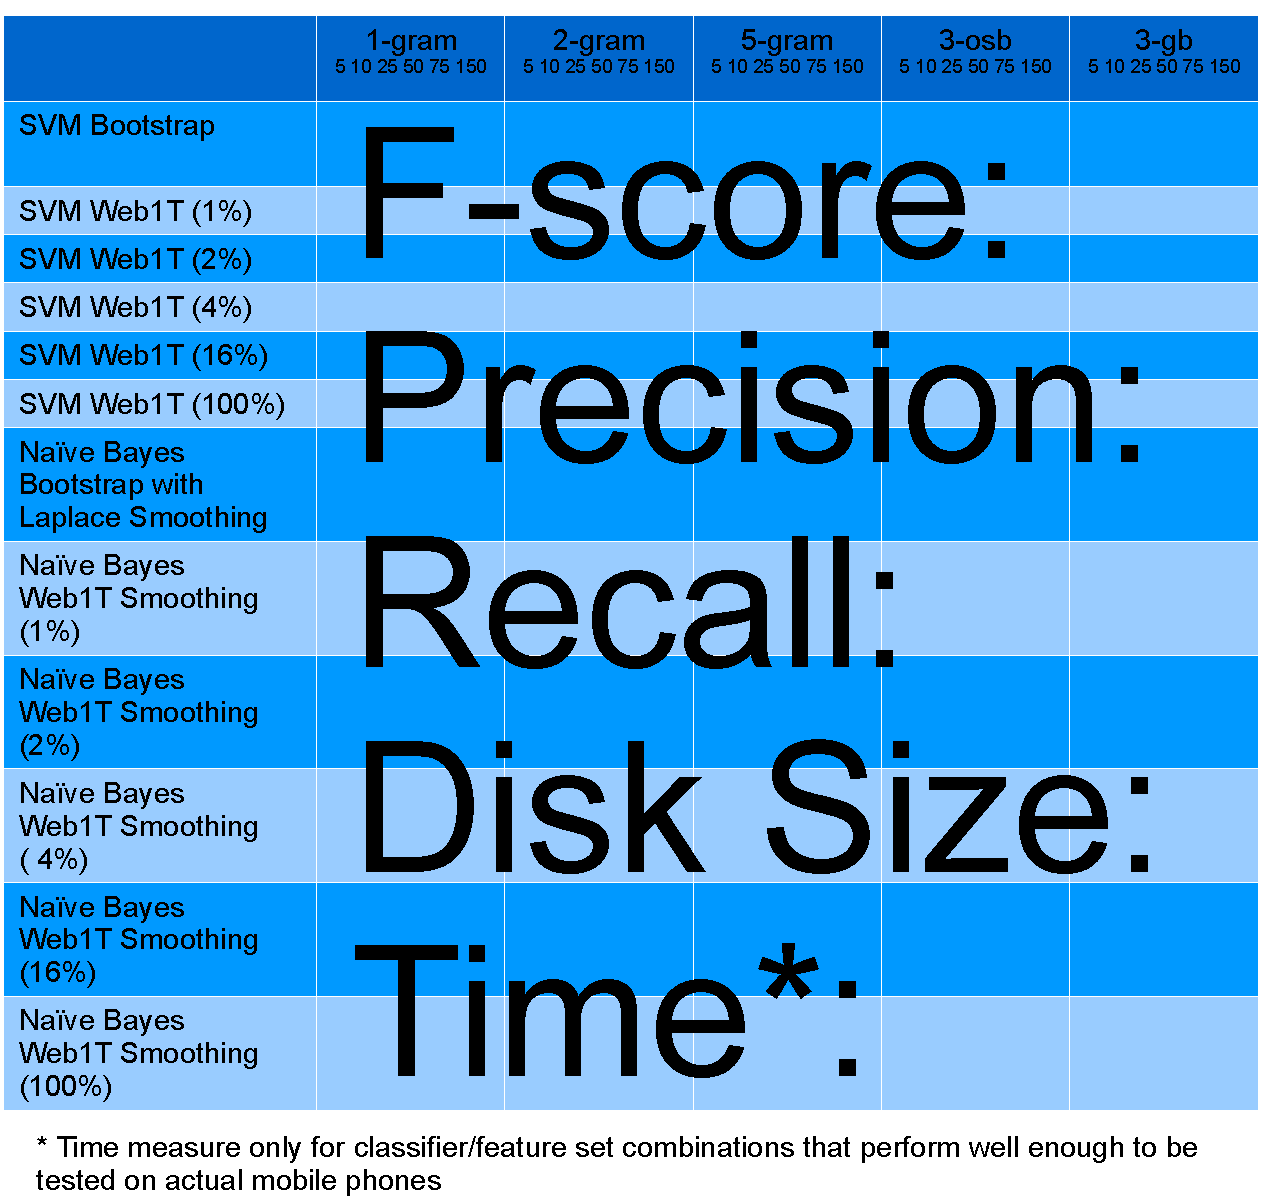
\includegraphics[width=0.5\textwidth]{Experiment_Design.pdf}}
			\caption{Parameter Combinations for Testing}
			\label{fig:parameterCombinations}
		\end{center}
	\end{figure}
	
The small numbers "5 10 25 50 75 150" given under each column heading in Figure \ref{fig:parameterCombinations} indicate that all authors will be tested in groups of 5, 10, 25, 50, 75, and 150 using three different grouping strategies: small-to-large, small-and-large, and random. In small-to-large, the authors with the smallest amount of training data are grouped together.  In small-and-large, small authors and large authors are paired together.  In the random grouping, the authors are grouped together by a pseudo-random selection.  The reasoning for these three grouping strategies is to provide insight into the effect of prolific authors versus less prolific authors.  If results are similar for the same author for each group, the prolific writing may not impact the outcome of author detection with these methods.  This is needed information to rule out that the test author detection methods simply select the most prolific author instead of the actual author.

	\subsection{Organizing and Compressing Feature References} A key element to this testing is the use of the Google Web1T corpus.  The Web1T corpus contains billions of types with a token mass of just over 1 trillion.  The size and breadth of the Web1T corpus makes it appealing as a source for smoothing in Naive Bayes and a tool for creating models in SVM. However, due to the huge size of the Web1T corpus, the text files comprising the corpus must be compressed and managed for use on desktop workstations, servers, and especially mobile devices.  Managing the corpus requires determining what portions of the Web1T corpus will be used.  Using the choice of 5-grams as an example for illustration purposes, suppose only the 5-grams portion of the Web1T corpus might be used.  The 5-grams constitutes 118 text files containing up to 10 million lines of text each. Each line of the Web1T 5-gram files contains space separated words (making up the type) followed by a count, separated from the words by a tab.  The lines of text are organized alphabetically by token where uppercase letters are distinct from lowercase letters. Even using only one size of gram from Web1T, a reverence of this size is slow and bulky for machine learning use.  Therefore, a subset of the reference is needed.
		\paragraph{Sizing the Feature Reference Set} To manage the size of Web1T, a small portion of the 5-grams could be chosen -- 1\%, 2\%, 4\%, etc.  To choose which part of the reference to use (largest, smallest, random) this thesis takes advantage of Zipf's Law.  Zipf's law states that the highest frequency word occurs approximately twice as often as the next most frequent word.  By that reasoning, a list of the types with the highest counts is needed to capture the largest use of words in a natural language corpus.  To get this count ordered list, the complete set of Web1T n-grams are recreated.  The recreated files list each type organized by count instead of alphabetically.  If two or more types have the same count, then those types are list alphabetically.  The types are still listed first as a group of space separated words followed by a tab and ended with a count.

		\paragraph{Three Tiered Hashing Scheme} Even once the feature set of types to be used for classification has been determined, the smaller set of text is still too slow to process and very bulky to store.  To further compress the data, a three tiered hashing scheme is used.  The structure of the three tiered hashing scheme is shown in Figure \ref{fig:3tierHashStructure}. 
		
		\begin{figure}[h!]
			\begin{center}
				\fbox{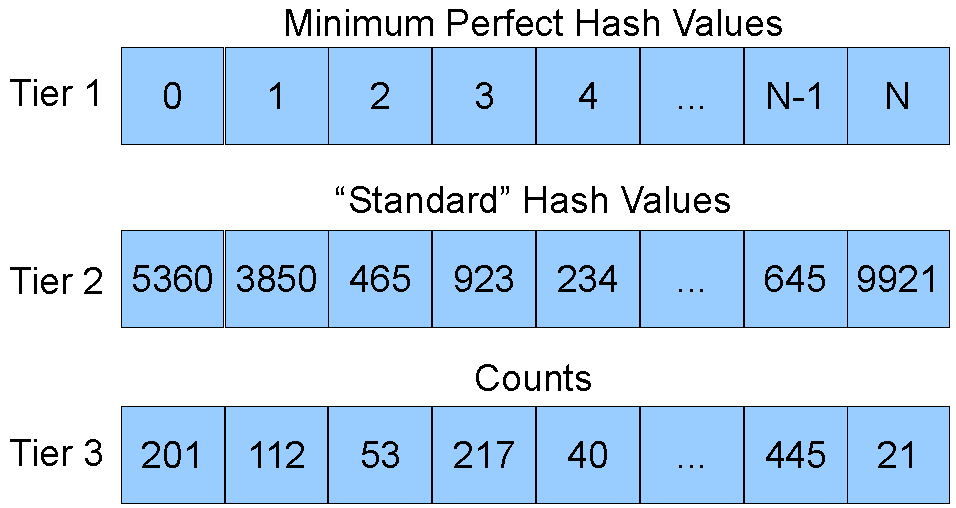
\includegraphics[width=0.75\textwidth]{3_tier_explanation.pdf}}
				\caption{Three Tiered Hashing Scheme Structure}
				\label{fig:3tierHashStructure}
			\end{center}
		\end{figure}
		
		The first tier is comprised of minimal perfect hash (MPH) values of the selected feature set.  The second tier of the scheme is comprised of a 64 bit hash of the original type.  This second tier's job is to reduce the probability of a false positive in the fist tier.  This issue arises because no matter what string is input to the MPH function, a valid MPH value will be produced.  The second tier's traditional hash is accessed by mapping the MPH value to the index of an array that comprises the second tier.  That array cell contains the 64 bit hash of the original text used to create the MPH value.  This make the false positive rate for a given type $\frac{1}{2^{64}} * \frac{1}{\text{range of MPH values}}$ which is deemed an appropriate risk of collision in this hashing scheme.  The third tier is simply an array of long values.  The MPH value from tier 1 is used to access this array which hold the count value for a given type.  An example of converting a phrase, "the quick brown", is shown in Figure \ref{fig:3tierHashExample}. 
		
		\begin{figure}[h!]
			\begin{center}
				\fbox{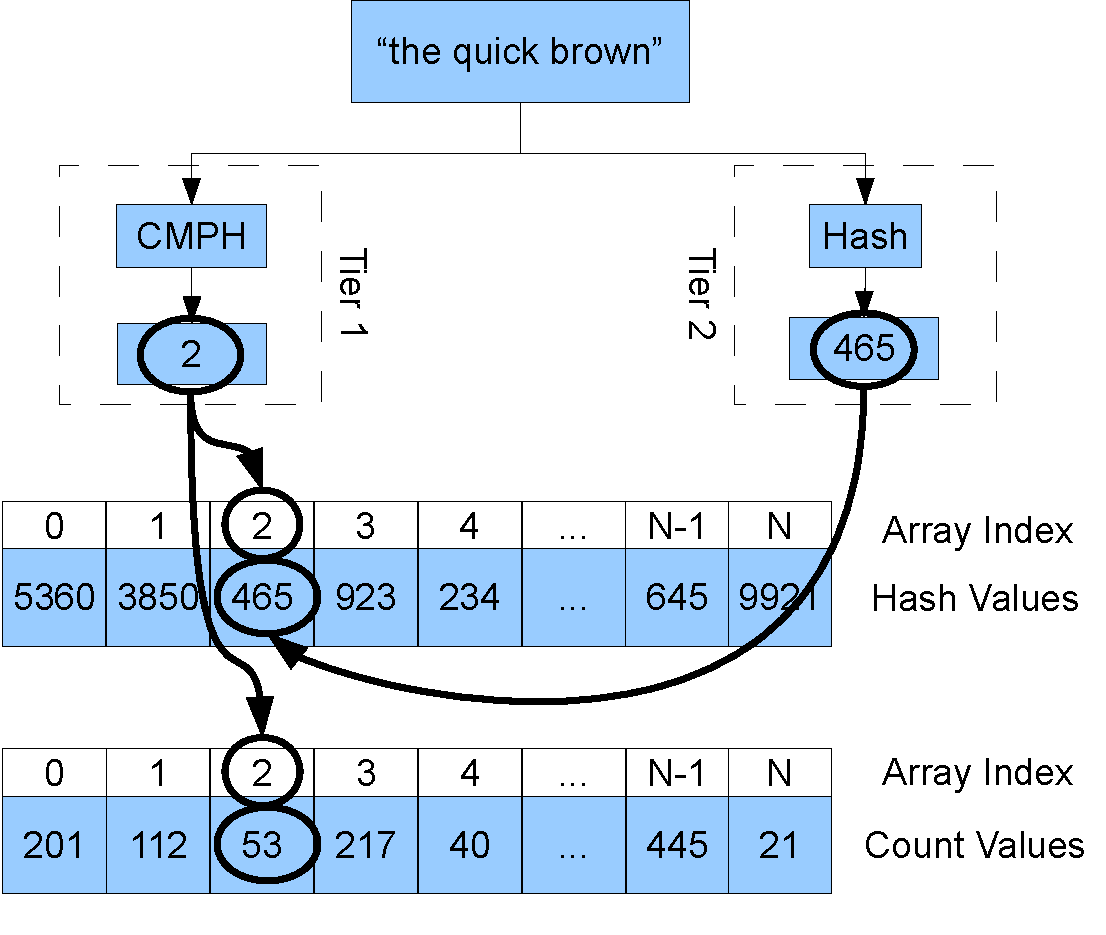
\includegraphics[width=0.75\textwidth]{3_tier_example.pdf}}
				\caption{Three Tiered Hashing Scheme Example}
				\label{fig:3tierHashExample}
			\end{center}
		\end{figure}
		
		These different tiers are not contained in a single data structures.  The MPH data structure, tier 1, is contained in a file called "keys.mph".  The array of hash values, tier 2, is contained in a file called "signature".  The counts are contained in a Java object file call LongCountsArrayFile.  The Naive Bayes experiments use all three tiers of this structure for smoothing values.  The SVM experiments only use tier 1 and tier 2 to verify that a string encountered actually belongs to the feature set.  These hefty data files comprise the bulk of storage required on the mobile device.  Since these data files get loaded into RAM during the prediction process, the file sizes also impact RAM requirements. The impact on RAM and disk storage makes management of the size of keys.mph, signature, and LongCountsArrayFile an important aspect of the experiments.

		\paragraph{Choosing Artifacts for the Three Tiered Hashing Scheme} One impact of using MPH to reduce the size of storing types is a loss of flexibility with the text artifact selection process.  Before the MPH data structure is created, the creator must determine if punctuation, capitalization, sentence boundaries, or "unknown" words will be allowed.  The omission of each of these artifact types brings its own unique challenges. A binary style number scheme was adopted for each of these features where capital letters hold the 1 position, punctuation the 2 position, unknown word tags the 4 position, and sentence boundaries hold the 8 position.  The complete matrix of artifacts allowed in the MPH model is included in Figure \ref{fig:cmphMatrix}.
		
		\begin{figure}[h!]
			\begin{center}
				\fbox{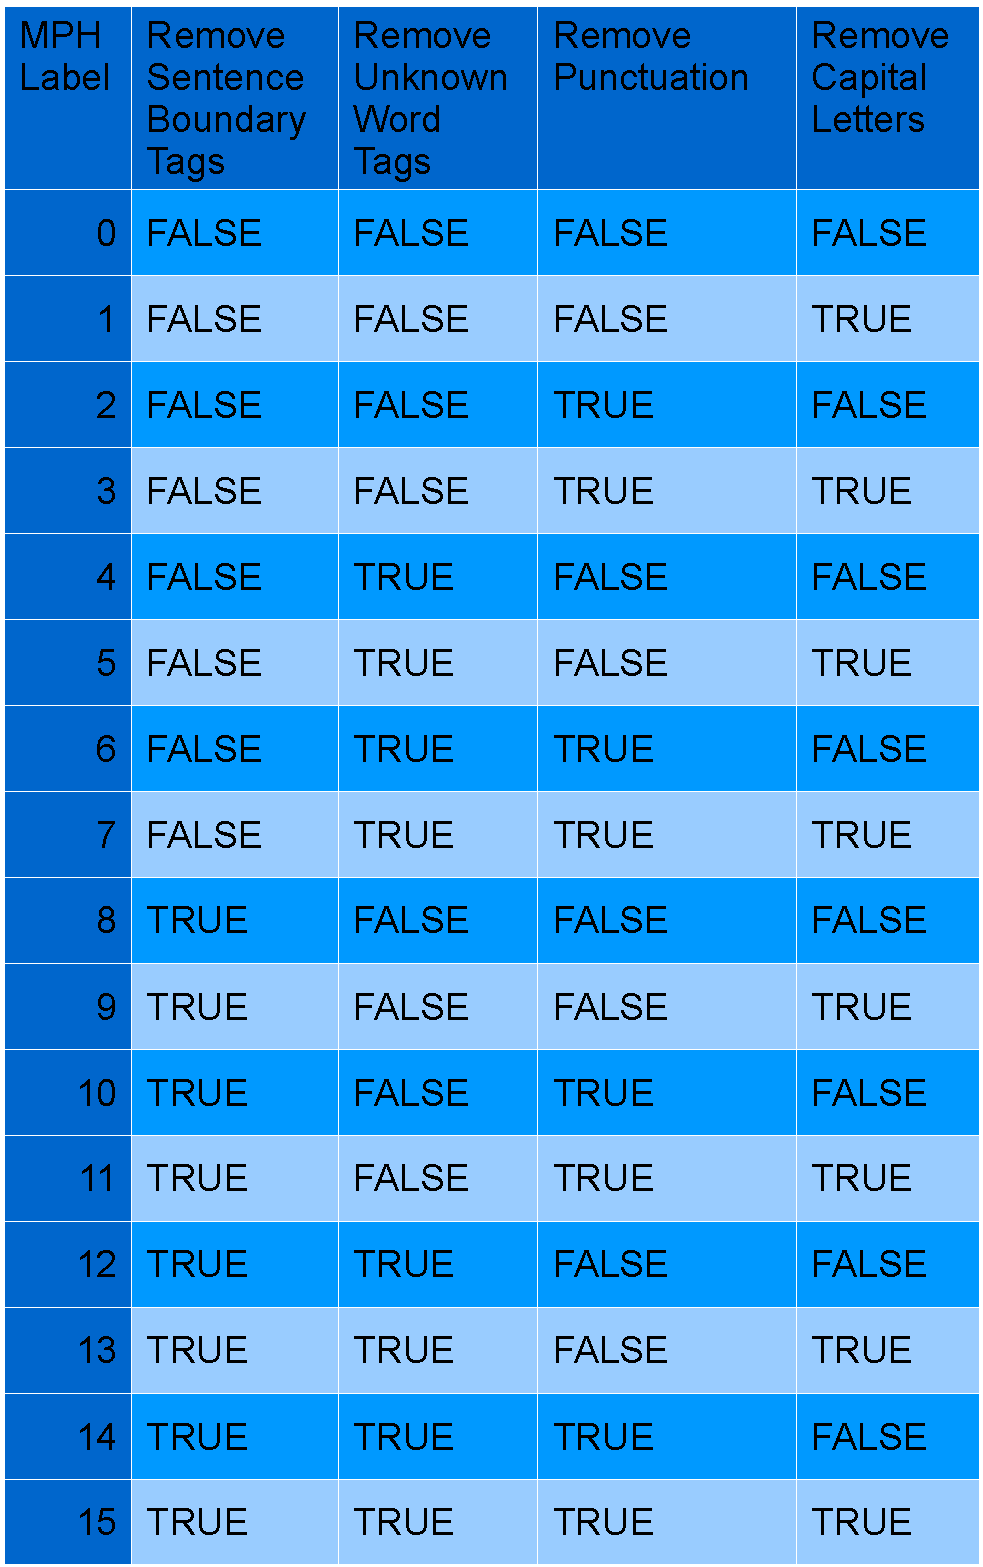
\includegraphics[width=0.5\textwidth]{cmph_matrix.pdf}}
				\caption{Matrix of CMPH Models by Artifacts Included}
				\label{fig:cmphMatrix}
			\end{center}
		\end{figure}
		
			\subparagraph{Omitting Punctuation} Omitting punctuation provides two options for dealing with the corpus: replace punctuation with "$<\text{UNK}>$" or drop the punctuation altogether.  If punctuation is dropped, then any type containing a punctuation mark in the feature reference set must be completely ignored.  If the punctuation is replaced with $<\text{UNK}>$, then a search within the existing count structure must be conducted for a corresponding entry for $<\text{UNK}>$ and any non-punctuation words in the type.  While dropping punctuation is much simpler to implement than employing "$<\text{UNK}>$" tags, however, Google did count punctuation as a word in type construction, so correlation between n-gram counts in the Web1T corpus and the trained/predicted documents is slightly affected. To maintain simplicity, the simple drop approach was used in these experiments.
			\subparagraph{Omitting Capitalization} Omitting capitalization is straightforward for construction of tier 1 and tier 2, the inputted text for the type is converted to all lower case and a check is conducted to see if that type is already in the MPH data structure.  For tier 3, which contains the counts, the lower case versions of the word must have its count mass added with its corresponding uppercase types.  This adds complexity to the insertion process for MPH but is easily managed.  Another option would be to simply drop all types that contained capitalization, but that would remove a large count mass from the Web1T corpus.  Adding counts was the method used in this thesis to deal with omitting capitalization.
			\subparagraph{Omitting Sentence Boundaries}  Sentence boundaries are denoted in the Web1T corpus as $<\text{S}>$ and $<\backslash \text{S}>$. Dropping sentence boundaries is straightforward since there is no replacement or count mass issues to deal with.  Since the tools for locating sentence boundaries make use of their own machine learning processes, no sentence boundaries were used in these experiments.
			\subparagraph{Omitting Unknown Words} In the Web1T corpus, "unknown" words have a specific meaning.  To be included in any corpus n-gram set, a word must have appeared as a 1-gram at least 200 times in the Google database.  By contrast, to be 2-gram, 3-gram, 4-gram, or 5-gram, that gram had to appear at least 40 times in the Google database.  This created as situation where a word would need to appear in a 2-or-higher-gram, but was not allowed into the corpus because it did not appear 200 times in the overall database.  Words that fall into that category are replaced with the tag $<\text{UNK}>$ in the Web1T corpus.  Removing $<\text{UNK}>$ words from the MPH has no effect on the counts in tier3 and is a straightforward process.
		
		\paragraph{Choosing N-Grams} N-grams can be as small as a 1-gram and grow, theoretically, to any size N imaginable.  The preferred reference set for this thesis, the Web1T corpus, uses 1, 2, 3, 4, and 5-grams.  While it is tempting to test all 5 N-gram sizes available in the corpus, only three were used.  1-grams and 5-grams were chosen to represent opposite ends of the size N gram spectrum available.  2-grams were used as a strong comparison to gappy bigrams and orthogonal sparse bigrams discussed below.  Future work could focus on 3 and 4-grams to determine if there is a performance to size advantage in using those size of N-grams.
		
		\paragraph{Gappy Bigram and Orthogonal Sparse Bigram Construction} Once the 3 tier structure is created and functional, there are still two type of features remaining to be created.  The Web1T corpus only contains standard n-grams, not gappy bigrams or orthogonal sparse bigrams.  To create these more exotic types of bigrams, a rule for counting distance and a notation scheme was needed.  It was decided to use "lesser included counts" for both the gappy bigrams and the orthogonal sparse bigrams.  This means that a word1 word2 pair would count for osb-0, osb-1, osb2, etc.  While previous papers placed the distance for an OSB between word1 and word2 \cite{bikel_if_2007}, this thesis constructed the OSBs with the distance after word2 for easier parsing.  The gappy bigrams and OSBs were constructed from the 2, 3, 4, and 5-grams in the Web1T Corpus.  Word pairs from a distance of 0 (a traditional bigram or an OSB-0) to a distance of 3 (an OSB-3 or the first and last word in a 5-gram) were built from the Web1T corpus.  This process only looks at the first and last words in a 3-gram, 4-gram, or 5-gram since the inner words of this gram are already captured in the 2-gram.  Using the inner 2-grams would double count 2-grams and throw off the count mass.  The same is true for 3-grams inside of 4 and 5-grams as well as 4-grams inside of 5-grams.
	
	\paragraph{Grouping By Size} With references built and sized, an efficient structuring of the authors and documents needs to be devised.  During data file construction, the grouping and conversion processes happened simultaneously.  The grouping sets built were: small-to-large, small-and-large, and random.  
		\subparagraph{Small-To-Large} The small-to-large group matched the least prolific authors together with increasing size up to the most prolific authors.  For example, of the 5 authors in the ENRON corpus with 5 total kilobytes worth of text are group together while the 5 authors with greater than 1 total megabyte of text are group together.  No author is picked more than once.  An example is shown in Figure \ref{fig:smallToLargeGrouping}.
		\begin{figure}[h!]
			\begin{center}
				\fbox{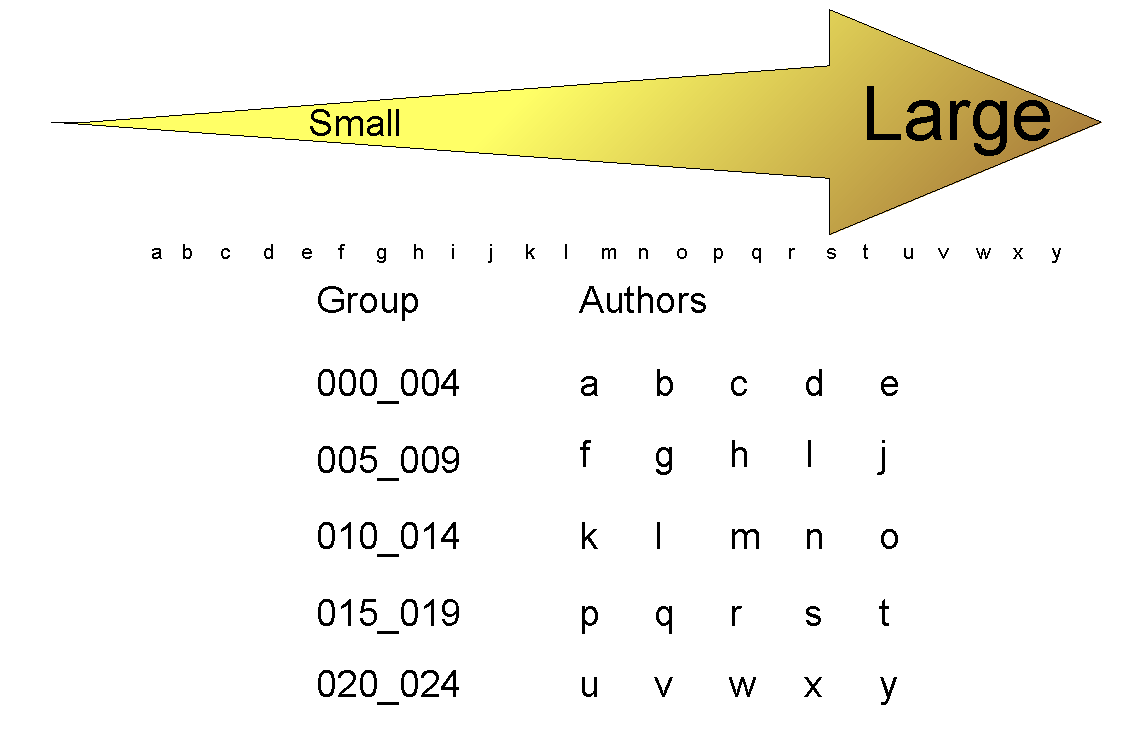
\includegraphics[width=0.5\textwidth]{small_to_large_grouping.pdf}}
				\caption{Small-To-Large Group for Group Size 5, 25 Authors}
				\label{fig:smallToLargeGrouping}
			\end{center}
		\end{figure}
		\subparagraph{Small-And-Large} The next group, small-and-large, is created by binning the authors by size.  Then one author from each bin is picked to be group with one author from each other bin.  For example the least prolific author is paired with one author from the most prolific bin and one author from each bin in between.  In this situation, the selection from each bin is not random.  The least prolific remaining author from each bin is picked for grouping.  No author is picked more than once. An example is shown in Figure \ref{fig:smallAndLargeGrouping}.
		\begin{figure}[h!]
			\begin{center}
				\fbox{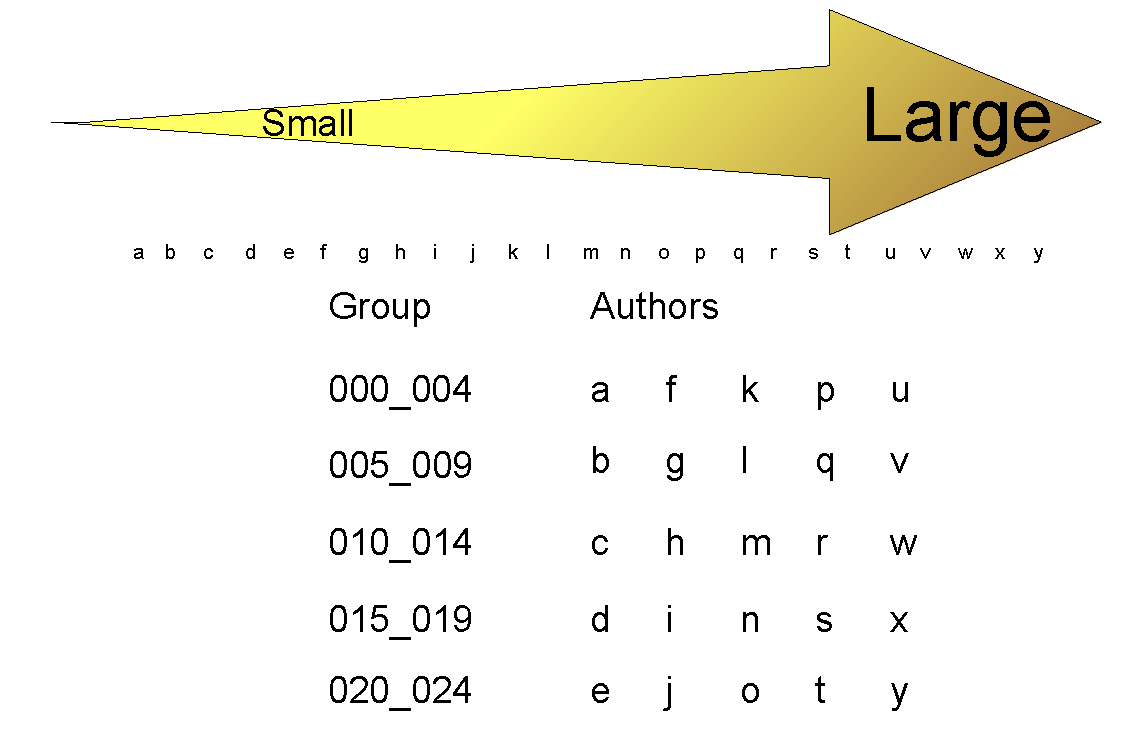
\includegraphics[width=0.5\textwidth]{small_and_large_grouping.pdf}}
				\caption{Small-And-Large Group for Group Size 5, 25 Authors}
				\label{fig:smallAndLargeGrouping}
			\end{center}
		\end{figure}
		\subparagraph{Random} This grouping simply produces a random number in the range of available authors and places the selected author into a group until that group is full.  Then the next group is filled the same way until no authors remain.  No author is picked more than once. No author is picked more than once. An example is shown in Figure \ref{fig:randomGrouping}.
		\begin{figure}[h!]
			\begin{center}
				\fbox{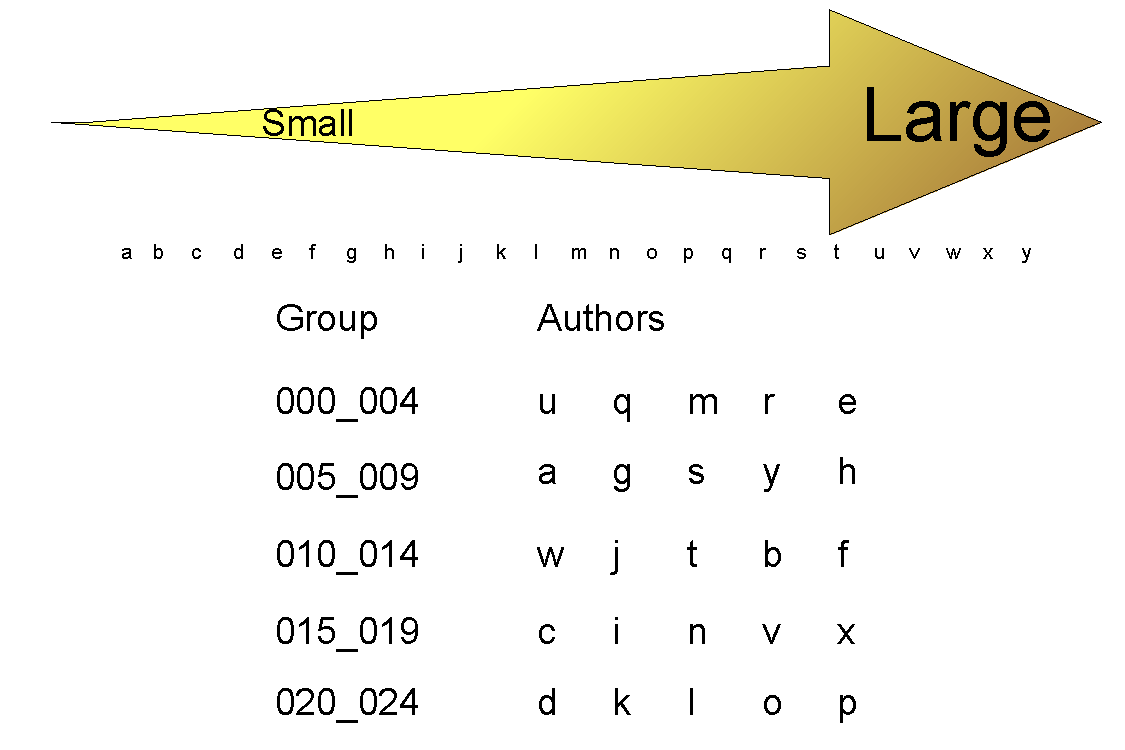
\includegraphics[width=0.5\textwidth]{random_grouping.pdf}}
				\caption{Random Group for Group Size 5, 25 Authors}
				\label{fig:randomGrouping}
			\end{center}
		\end{figure}
		\subparagraph{Group Sizes} Based on having 150 authors in the ENRON Corpus, the six following group sizes were used: 5, 10, 25, 50, 75 150.  These six group sizes coupled with the three grouping types, small-to-large, small-and-large, and random creates 18 grouping types.  Examples of these grouping types are 5 small-to-large, 5 small-and-large, 5 random, 10 small-to-large, ..., 150 small-to-large, 150 random.  Although using all 150 authors in a grouping set makes the procedure of how the 150 were grouped redundant, all three size 150 tests were conducted as a check on the experiments. If the 150 author grouping provides different reslts, then there may be an issue with the classifiers.
		\subparagraph{}After these grouping types were constructed, there were 171 totals sets (30 sets of 5 small-to-large, 15 sets of 10 small-to-large, ..., 1 set of 150 small-to-large, 1 set of 150 random.)  Each of these sets were intended to be run through Bootstrapped SVM, Web1T SVM, Laplace Smoothed Naive Bayes, and Web1T Smoothed Naive Bayes.  Assuming that only one MPH model is chosen to represent Google Web1T, that results in 684 experiments.  Since there are 16 different MPH models based on the combinations punctuation, capitalization, sentence boundaries, and unknown words, the number of experiments could rise drastically.  However, only two MPH models will be used during the experiments resulting in only 1,368 per feature type.  Using 1-grams, 2-grams, 5-grams, 3-gb, and 3-osb results in 6,840 totals experiments.
	
		\paragraph{Data File Format}With combinations of features, artifacts, and group sizes chosen and the MPH data structures created, the actual documents must be converted into a format that can be used by the classifiers. The LibSVM file format was used since that it is the native format for LibLinear, the tool used for SVM in this thesis.  The Naive Bayes classifier was built specifically for this thesis and was designed to use LibSVM format for convenience. The format of the data files consisted of an integer representing the author followed by a space, followed by a number representing the MPH value, followed by a colon, followed by another number representing the count.  Each succeeding instance of a MPH value coupled with a count is separated by a space.  Each document in the corpus is represented by a single line.  Each line's mph number is in increasing order from left to right.  The data files store the word/count pairs in a sparse fashion.  This means that a zero count is not included in the data file.  Absence of a word/count pair constitutes a zero count without needlessly using up space in the file.  An example of this file format is provide in Figure \ref{fig:svmFormat}.
		\begin{figure}[h!]
			\begin{center}
				\fbox{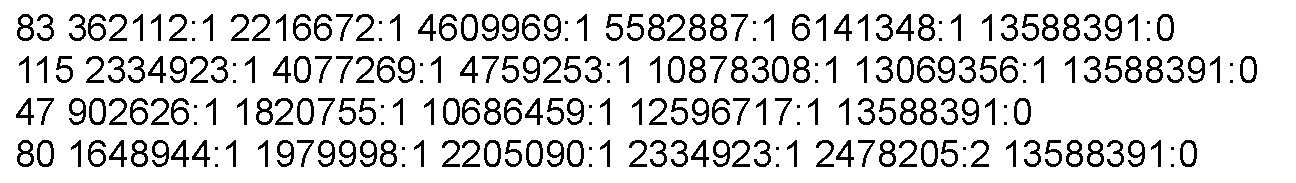
\includegraphics[width=.75\textwidth]{svm_format.pdf}}
				\caption{LibSVM File Format}
				\label{fig:svmFormat}
			\end{center}
		\end{figure}
	
	\paragraph{Running SVM} With the data files created, the classifiers can be applied. The chosen tool for author detection using SVM is LibLinear.  LibLinear was chosen for its speed compared to LibSVM.  The LibLinear source code was slightly modified to allow training a model from a data set, then running prediction on a separate set without using the built-in cross validation function.  During the training phase, each author has a SVM model built for it from a training file in a directory labeled "train".  During the prediction phase, document contained in another file are used to predict the mostly likely author.  That file is contained in a folder called "predict". The SVM author result is printed to a result file in a directory labeled "result".  The f-score, precision, and recall for each file is recorded in a file inside a folder labeled "analysis".  The analysis file also contains a full confusion matrix, time of prediction, size of original file, and other statistics.  This file is finally pulled into a mySQL database for storage and calculation of precision, recall, and f-score..
	\subparagraph{} The size of the author models impacts RAM usage and disk space.  LibLinear stores SVM models as an array. RAM and storage are not the only limits.  An array of integers representing token counts can be sizable, especially when token counts are long numbers (64 bits) instead of integers (32 bits). 
	\subparagraph{} RAM and disk storage are not the only limits. By specification, arrays in Java are limited to $2^{31}-1$ entries.  This means the model cannot contain more than $2^{31}-1$ features.  Also, the model must be loaded into RAM, so the number of authors coupled with the size of the author model must be weighed against the available RAM and disk storage.
	
	\paragraph{Running Naive Bayes} The Naive Bayes classifier has been specifically built for this thesis.  The classifier reads in a pre-built array of long values from a file.  The two types of arrays are a Laplace Smoothing array, which is comprised of all 1's.  the second type of array is the Google Smoothing array comprised of the count values from the Web1T corpus.  Using an array to hold the smoothing values for Naive Bayes has an impact on RAM usage.  There must be enough available RAM to hold the smoothing array.  To prevent having numerous copies of the smoothing array in memory (one for each author being trained) a hashmap is used to create the author models instead.  The process for training put each encountered feature type into a hashmap along with a count of $1 plus \text{the array smoothing value}$.  If that feature type is encountered, the the count is simply incremented. Once all the training documents have been read and counted, the hashmaps of feature types and counts is converted into a hashmap of feature types and log of probability.
	\paragraph{}During the prediction process, each encountered feature type is queried against the author hashmap first.  If the feature type is found in the hashmap, then the hashmap $\log{probability}$ is used.  If not, then the smoothing array containing log of probabilities is used.  An example of this hashmap/array process is shown in Figure \ref{fig:predictionFlowChart}. The result of the prediction process is outputted to a file in the corresponding results directory.  Those results are then processed into a file in the corresponding analysis folder where all data is then read into a mySQL database for evaluation of precision, recall, and f-score.
		\begin{figure}[h!]
			\begin{center}
				\fbox{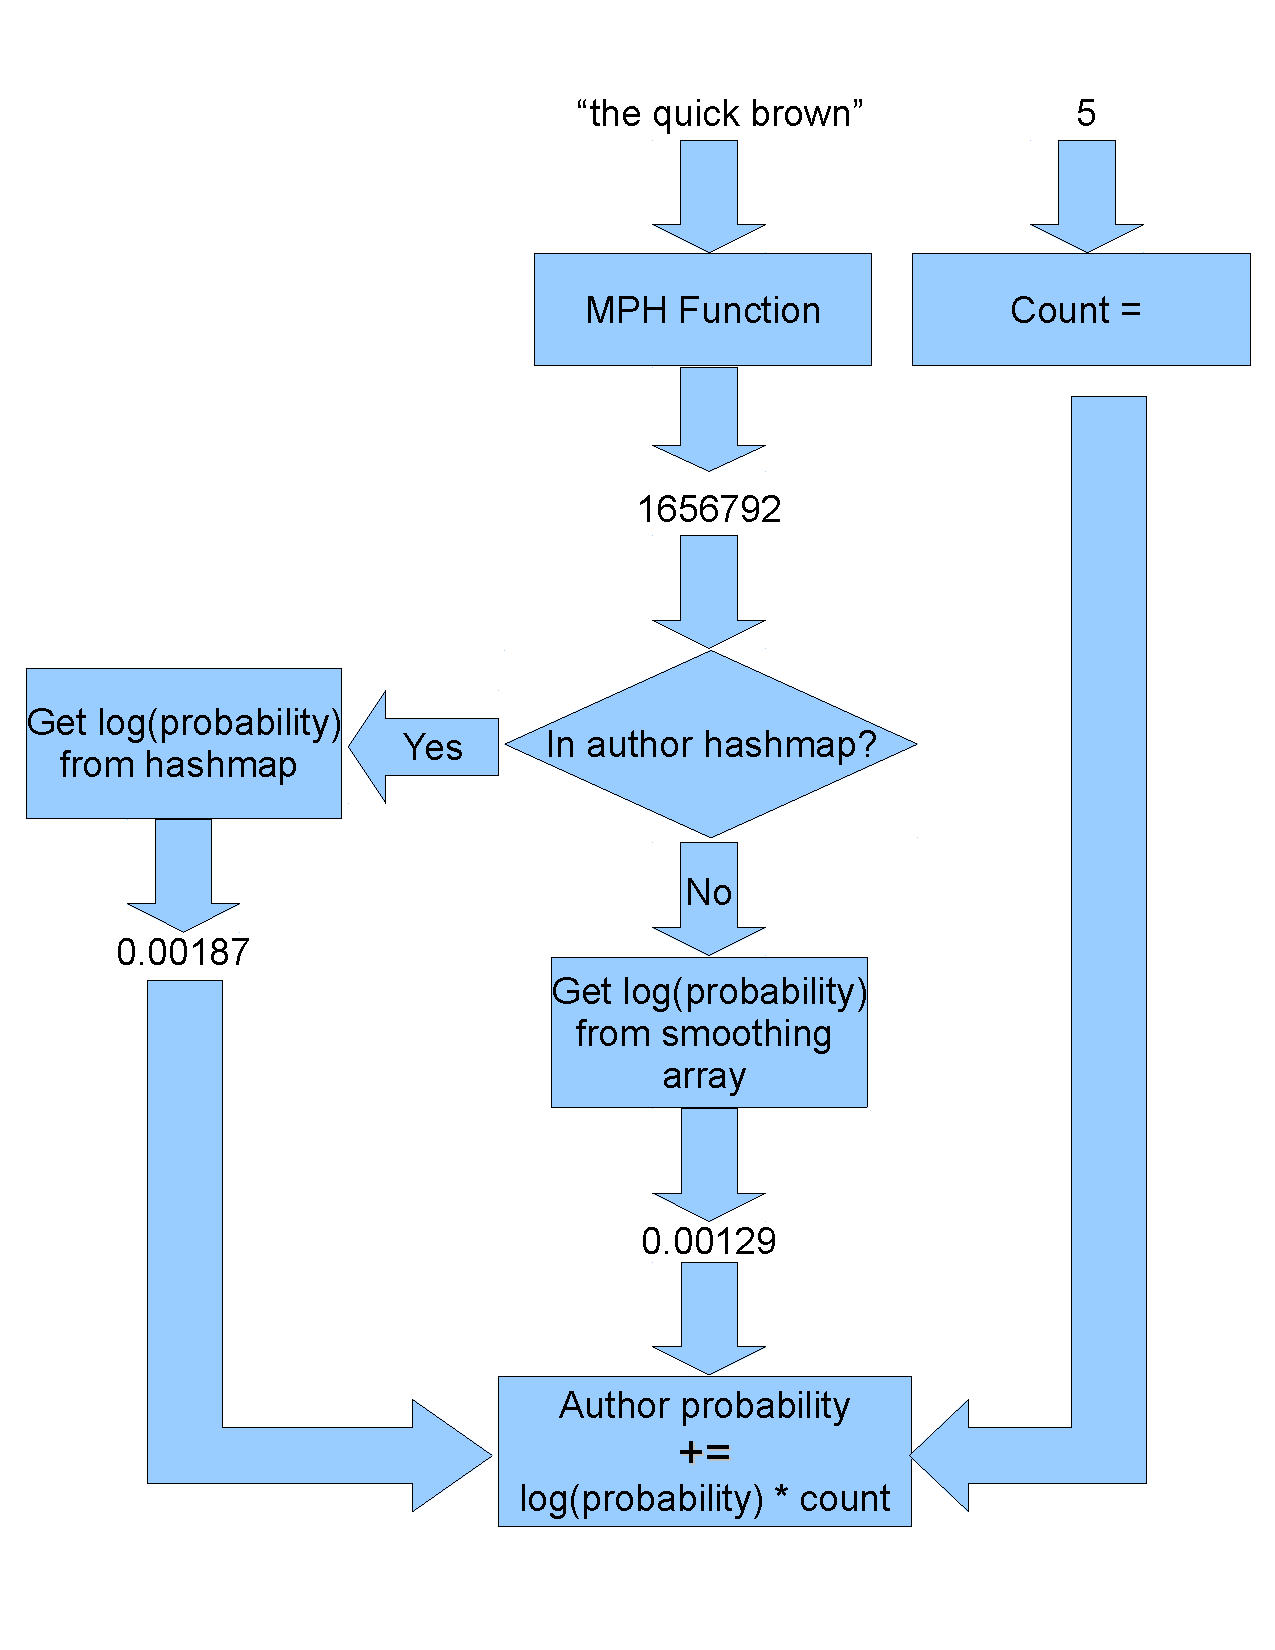
\includegraphics[width=.75\textwidth]{prediction_flow_chart.pdf}}
				\caption{Naive Bayes Hashmap and Smoothing Array Flow Chart}
				\label{fig:predictionFlowChart}
			\end{center}
		\end{figure}

%\section{Experiment Design}
%	\paragraph{}The objective of the experiments in this thesis are to populate a table of key metrics regarding author detection on a mobile phone.  The keys metrics are f-score, precision, recall, size on disk, %size in RAM, CPU consumption, and time required.  These metrics are aimed at the process of predicting the author, not at the process of training for the authors.  All author detection model training will be conducted on a workstation or server, not on a mobile phone.  The experiment will use a variety of combinations of feature sets, classification methods, and user set sizes.  The specific combinations are given in ;adslkfjads;lfkjads;lfk below:
%	\begin{center} 
%		Corpora
%		\begin{itemize}
%			\item ENRON Email Corpus
%			\item Naval Postgraduate School Twitter Corpus
%		Classification Methods
%		\begin{itemize}
%			\item Naive Bayes with Laplace Smoothing
%			\item Naive Bayes with Google Web1T Count Smoothing
%			\item Support Vector Model bootstrapped from training set
%			\item Support Vector Model with Google Web1T Types for dimensions
%		\end{itemize}
%		Feature Sets
%		\begin{itemize}
%			\item 1-grams (unigrams)
%			\item 2-grams (bigrams)
%			\item 5-grams
%			\item 3-gappy bigrams
%			\item 3-orthogonal sparse bigrams
%		\end{itemize}
%		User Set Size
%		\begin{itemize}
%			\item all versus all (mutlicalss
%			\begin{itemize}
%				\item 5 users
%				\item 10 users
%				\item 25 users
%				\item 50 users
%				\item 75 users
%				\item 150 users
%			\end{itemize}
%			\item one versus all
%			\begin{itemize}
%				\item 5 users
%				\item 10 users
%				\item 25 users
%				\item 50 users
%				\item 75 users
%				\item 150 users
%			\end{itemize}

%\paragraph{}The two classifiers chosen were Naive Bayes and Support Vector Model.  While there are many classifier tools available, these two methods were chosen for nominally being on the opposite end of the simplicity and effectiveness scales.  For text classification tasks, Naive Bayes is often less effective than SVM.  Naives Bayes is simpler to implement than SVM, so the tradeoff is simplicity versus effectiveness.  Naive Bayes is much lighter on CPU usage and time than SVM.  Both Naive Bayes and SVM can process training and predicting files in a sparse format, which saves on disk storage.  Naive Bayes must deal with zero probabilities stemming from a lack of training data to make the Bayes equation work out to something other than zero, and, more importantly, smoothing lessens the impact of the spiky nature of discrete data.  This smoothing is intended to provide a more reliable result.  For SVM, the SVM model can be created by only accepting words found in the actual training data or the features can be created from a feature reference, such as Google Web1T.  In the case of using a feature reference, SVM simply puts a value of 0 for each feature not provided a number in the training or prediction data.
%\section{Program Design}
%	\paragraph{}Write a cmph module to transform strings of words into numeric values.  Store those values in a file.  Have this module account for sentence boundaries, punctuation, capitalization, and unknown words.
%	\paragraph{}Transform corpus documents from a set of strings to a set of cmph created values, a different document corresponding to each cmph model (punctuation, .  Store the corpora in cmph numeric form.

%\section{Data Management}

\section{Phase Two: Android Implementation}
	\paragraph{}To manage files on the mobile device, a rudimentary file manager was built with a text viewer added.  A button was also added to the File Manager to execute prediction against a document on the phone.  An Android Service was also constructed that listens for incoming SMS messages.  When an SMS Message is "heard", it is processed for author detection.  The Service can be turned on and off using a button on the File Manager.  
	\paragraph{}To measure CPU and RAM impact caused by the author detection processing, the third party applications, and Memory Usage, was installed on the phones.  The method is to take a baseline of the phone's CPU and RAM usage with no Widgets or Applications running, the phone is attached to a recharging device, and no calls or texts are being sent.  The same phone conditions are being set for the processing tests where the only application that will run on the phone will be the SMS capture and author detection application for this thesis.  This will yield some basic metrics of author detection impact on the phone's capabilities.

\section{Corpora} Two corpora are used for this thesis: the ENRON Email Corpus and the Naval Postgraduate School (NPS) Twitter Corpus.  The aim of this thesis is to examine author detection using a mobile device.  Two of the most common text communications on a mobile device are email and SMS (texting).  The ENRON Email Corpus has been widely examined and has been used to author attribution in other studies.  This makes the ENRON Corpus a suitable standard to measure the author detection techniques used in this thesis.  The NPS Twitter Corpus is smaller and newer than the ENRON email corpus, but texting is extremely popular as a communications medium.  Determining the effectiveness of author detection over this rapidly expanding text standard is important for analyzing the effectiveness of author detection on mobile devices.
	\paragraph{ENRON Email Corpus} Each ENRON email was stored in a single text file within a folder labeled with the author's first initial, second initial, and last name.  Prior to processing each ENRON email, a systematic attempt was made to distill each email down into just the author's words.  To support this distillation, the email header was stripped from each email.  A search was conducted throughout the remaining text to find additional email headers.  These are the embedded headers caused by email replies and forwards.  Also to prevent biasing the author attribution, an attempt was made to systematically detect an email closing such as "Sincerely, Dave" or "Yours Truly, Jane".
	\paragraph{Naval Postgraduate School Twitter Short Message Corpus} All tweets from a single author were stored in a single text file.  Each tweet from that author was contained on its own line.  Each line begins with a date-time stamp with the content of the text following.  Prior to constructing the corpus, all "re-tweets" were removed to ensure the text came from a single author, not just from a single Twitter account.
	
\section{Intended Comparison}  Once all tests are complete, performance of the different combinations of feature and classifiers will be compared for both the ENRON email corpus and the Twitter Corpus.  This is to allow any differences in performance against the two primary media used on mobile phones.  The completed test results should provide insight into the possibility of author detection on a mobile phone against both email and short messages.




 % Experimental Design
\chapter{Results and Analysis}

	\paragraph*{} After 19,782 tests producing 286,050 measurements for f-score and 19,782 measurements for accuracy, several notable results emerged.  Most importantly, a small number of method-feature combinations do exist that both provide a reasonable author detection accuracy and have a storage requirement of less than 16MB.  Further, in studying the effects of using the Google Web1T Corpus, Web1T did not provide enough benefit to accuracy to justify its large storage requirement.  This does not mean that Web1T did not have a positive impact on accuracy, especially for the Enron corpus and naive Bayes.  It was also found that Web1T had different impacts on dissimilarly prolific authors than on similarly prolific authors. This chapter provides specific details about usable method-feature combinations and the impacts of Web1T.
	\paragraph*{} There is one notation convention used in this chapter that requires explanation.  The notation Web1T\% refers to the top percentage of the Web1T corpus used as the vocabulary in testing.  For instance, Web1T\% of 1 for OSB3 means that the top 1\% of orthogonal sparse bigrams of distance three (OSB3) were used as the vocabulary.  Web1T\% of 2 for GB3 means that the top 2\% of gappy bigrams of distance three (GB3) are used.  This pattern continues for Web1T\% of 4, 8, and 16 and feature types of 1-grams (GM1), 2-grams (GM2), and 5-grams (GM5).  The only special case is for Web1T\% of 0.  In this case, there was no reference to the Google Web1T Corpus at all in constructing the vocabulary.  The vocabulary is built using any and all tokens found in the training set.

\begin{singlespace}
\section{Most Effective Combination of Classification Methods, Feature Types, and Vocabulary}
\end{singlespace}
	\paragraph*{} Two measurements of effectiveness were used in this thesis: accuracy and f-score.  Since the accuracy for each author is not the focus of this thesis, but rather the overall effectiveness of each classifier, feature type, and vocabulary combination, f-score is averaged, over the set of authors, for each combination.  In each test set, average accuracy was higher than MLE.  Likewise, average f-score was always lower than average accuracy.

	\paragraph*{} At this point, it would be natural to simply compare the highest accuracy for each method-feature-vocabulary combination in the thesis and determine which combination performed best.  This analysis would be flawed.  Due to the underlying data structure in the libLinear model, there is an absolute maximum number, $2^{31}$, of elements allowed.  The libLinear tool creates one element created in its model for each feature-classifier combination.  This means that the number of for each author, there is a dedicated cell for each feature.  The data structure impact for the libLinear tool is array size become the number of authors multiplied by the number of features.  Array size in Java cannot exceed $2^{31}$. This limits the of features that can be used with libLinear for a given number of authors. Figure \ref{fig:FeatureVSsize} shows the value of each feature-vocabulary-group combination.  Cells highlighted in red cannot be used with the LibLinear model.  If only the top $2^{31}$ features from each Web1T\% was used, then large Web1T\% values would have identical features.  For instance, two very large set are OSB3 for Web1T\% of 8 and Web1T\% of 16.  If only the top $2^{31}$ features were used from each of these features sets, then both of these sets, which far exceed $2^{31}$ features, would hold the same $2^{31}$ features.  This would create identical results and provide no additional insight into the true performance of that vocabulary. Therefore, due to the data structure limitation of the libLinear tool, there will be no LibLinear results for feature-author combinations that require an array larger than $2^{31}$ elements in the libLinear model.  
	

\begin{figure}[htbp!]
	\begin{center}
	\centering
	\includegraphics[scale=0.9]{FeatureVSsize}
	\caption{Liblinear Limits Due to Vocabulary Size and Group Size}
	\label{fig:FeatureVSsize}
	\end{center}
\end{figure}


	\paragraph*{}  While libLinear is the chosen SVM tool for this thesis, the classifier method being test is SVM.  For the rest of this chapter, results will be analyzied by method instead of by tool.  For this reason, results will be discussed in terms of SVM and naive Bayes instead of in terms of libLinear and naive Bayes.

	\paragraph*{} The impact of this hard maximum is large vocabularies show a higher accuracy and f-score than smaller vocabularies.  This is not necessarily because the large vocabularies are more effective, but because the larger vocabularies do not have the lower accuracy and f-score outcomes of the large group sizes.  To illustrate this, the top twenty feature-method combinations are show in Table \ref{tab:enron-accuracy-filtered-ranked} for the ENRON E-mail Corpus.  The performance of each SVM OSB3-vocabulary combination is shown in Figure \ref{fig:plot-liblinear-enron-accuracy}. Using Table \ref{tab:twitter-accuracy-filtered-ranked} to evaluate accuracy would lead to a conclusion that SVM OSB3 has the best accuracy and f-score in this thesis.  However, plotting all OSB3 results for each Web1t \%  in \ref{fig:plot-liblinear-enron-accuracy} shows that all OSB3-vocabulary combinations perform along a similar curve.  The Web1T \% $ of 0$ is actually able to perform against all group sizes (5, 10, 25, 50, 75, and 150) and, thus, appears to perform worse than other OSB3s in the table, but clearly performs similarly from Figure \ref{fig:plot-liblinear-enron-accuracy}.  From this example, it becomes clear that simply using the table values in Appendix A through Appendix D provides an insufficient analysis.  A better analysis is provided by examining the plots in Appendix Q through Appendix T.  
	
\begin{figure}[htbp!]
	\centering
	\includegraphics[scale=0.75]{liblinear-enron-avg-by-group_size}
	\caption{Accuracy of SVM OSB3 for the ENRON E-mail Corpus}
	\label{fig:plot-liblinear-enron-accuracy}
\end{figure}
	
	\paragraph*{}It is important to note that this is not an issue for combinations using naive Bayes as a classification method.  However, naive Bayes did not outperform SVM in these tests, so a careful analysis of SVM using the plots in Appendix Q through Appendix T is required.

	\paragraph*{} By examining the plots in Appendix Q through Appendix T, a clear trend emerges that the bootstrapped models, meaning models that made no use of the Web1T corpus as a vocabulary reference) performed similarly for SVM to Web1T vocabularies.  In all cases, the bootstrapped SVM tests are usable for all group sizes.  In this case, a good comparison would be to drop all SVM combinations that are not usable for all group sizes, then compare these remaining SVM tests against all naive Bayes tests.  Since all naive Bayes tests were usable for all group sizes, this makes the comparison fair.
	
	\paragraph*{} After extracting out SVM tests that were not usable against all groups sizes, the highest accuracy method-feature combination show the most accurate results for the ENRON E-mail Corpus in Table \ref{tab:enron-accuracy-filtered-ranked}.  The highest accuracy method-feature combination show the most accurate results for the Twitter Short Message Corpus in Table \ref{tab:twitter-accuracy-filtered-ranked}.
	
	
	\begin{table}[htbp!]
			\begin{center}
			\begin{tabular}{ | r | r | r | r | r | r | r | }
			\hline
			\multicolumn{2}{|c|}{Combinations} & \multicolumn{5}{|c|}{Accuracy}\\
			\hline
			Method & Feature Type & Web1T \% & AVG & MIN & MAX & STDDEV\\ \hline 
			SVM & OSB3 & 0 & 0.8362 & 0.5106 & 0.9732 & 0.1043\\ \hline 
			NB & OSB3 & 16 & 0.8325 & 0.5213 & 0.9823 & 0.0890\\ \hline 
			NB & OSB3 & 8 & 0.8315 & 0.5213 & 0.9714 & 0.0893\\ \hline 
			NB & OSB3 & 4 & 0.8274 & 0.5197 & 0.9587 & 0.0924\\ \hline 
			SVM & GM2 & 0 & 0.8262 & 0.4824 & 0.9753 & 0.1087\\ \hline 
			SVM & GB3 & 0 & 0.8212 & 0.4787 & 0.9835 & 0.1121\\ \hline 
			NB & GB3 & 16 & 0.8195 & 0.5201 & 0.9674 & 0.0947\\ \hline 
			NB & GB3 & 4 & 0.8194 & 0.5340 & 0.9522 & 0.0941\\ \hline 
			SVM & GB3 & 1 & 0.8191 & 0.4731 & 0.9673 & 0.1110\\ \hline 
			SVM & GB3 & 2 & 0.8184 & 0.4765 & 0.9805 & 0.1113\\ \hline 
			NB & GB3 & 8 & 0.8172 & 0.5255 & 0.9782 & 0.0935\\ \hline 
			NB & OSB3 & 1 & 0.8126 & 0.3615 & 0.9574 & 0.1185\\ \hline 
			NB & OSB3 & 2 & 0.8095 & 0.3526 & 0.9575 & 0.1283\\ \hline 
			NB & OSB3 & 0 & 0.8058 & 0.5185 & 0.9592 & 0.0970\\ \hline 
			SVM & GM5 & 16 & 0.7918 & 0.3908 & 0.9676 & 0.1204\\ \hline 
			SVM & GM5 & 8 & 0.7872 & 0.3908 & 0.9513 & 0.1193\\ \hline 
			NB & GB3 & 2 & 0.7857 & 0.4790 & 0.9669 & 0.1166\\ \hline 
			SVM & GM5 & 4 & 0.7755 & 0.3908 & 0.9455 & 0.1241\\ \hline 
			SVM & GM1 & 4 & 0.7742 & 0.4006 & 0.9590 & 0.1212\\ \hline 
			SVM & GM1 & 8 & 0.7740 & 0.4074 & 0.9570 & 0.1223\\ \hline 
			SVM & GM1 & 0 & 0.7735 & 0.3776 & 0.9531 & 0.1222\\ \hline 

			\end{tabular}
		\caption{Highest Accuracy Method-Feature Type Combinations for the ENRON E-mail Corpus}
		\label{tab:enron-accuracy-filtered-ranked}
		\end{center}
	\end{table}
	

	
	\begin{table}[htbp!]
	\begin{center}
			\begin{tabular}{ | r | r | r | r | r | r | r | }
			\hline
			\multicolumn{2}{|c|}{Combinations} & \multicolumn{5}{|c|}{Accuracy}\\
			\hline
			Method & Feature Type & Web1t \% & AVG & MIN & MAX & STDDEV\\ \hline 
			NB & OSB3 & 0 & 0.5525 & 0.2320 & 0.8164 & 0.1339\\ \hline 
			NB & GB3 & 16 & 0.5327 & 0.2216 & 0.8216 & 0.1351\\ \hline 
			NB & GB3 & 4 & 0.5271 & 0.2190 & 0.8546 & 0.1375\\ \hline 
			NB & GB3 & 8 & 0.5256 & 0.2176 & 0.8474 & 0.1362\\ \hline 
			NB & GB3 & 2 & 0.5249 & 0.2186 & 0.7823 & 0.1324\\ \hline 
			SVM & GM2 & 4 & 0.5228 & 0.1809 & 0.8210 & 0.1477\\ \hline 
			NB & GB3 & 1 & 0.5204 & 0.2148 & 0.8125 & 0.1319\\ \hline 
			NB & GB3 & 0 & 0.5203 & 0.1973 & 0.8021 & 0.1389\\ \hline 
			SVM & GM2 & 1 & 0.5197 & 0.1882 & 0.8454 & 0.1483\\ \hline 
			SVM & GM1 & 8 & 0.5187 & 0.1743 & 0.9026 & 0.1525\\ \hline 
			SVM & GM2 & 2 & 0.5186 & 0.1830 & 0.8232 & 0.1495\\ \hline 
			SVM & GM1 & 1 & 0.5159 & 0.1768 & 0.8211 & 0.1494\\ \hline 
			SVM & GM1 & 4 & 0.5149 & 0.1874 & 0.8546 & 0.1485\\ \hline 
			SVM & GM1 & 0 & 0.5141 & 0.1802 & 0.8089 & 0.1485\\ \hline 
			NB & GM1 & 0 & 0.5140 & 0.1247 & 0.7714 & 0.1631\\ \hline 
			SVM & GM1 & 16 & 0.5134 & 0.1865 & 0.8324 & 0.1483\\ \hline 
			SVM & GM1 & 2 & 0.5131 & 0.1818 & 0.8966 & 0.1487\\ \hline 
			SVM & GM5 & 1 & 0.4768 & 0.1398 & 0.8362 & 0.1521\\ \hline 
			NB & GM2 & 0 & 0.4750 & 0.1630 & 0.7890 & 0.1406\\ \hline 
			NB & OSB3 & 2 & 0.4739 & 0.1790 & 0.7734 & 0.1370\\ \hline 
			NB & OSB3 & 8 & 0.4707 & 0.1787 & 0.7790 & 0.1373\\ \hline 

			\end{tabular}
		\caption{Highest Accuracy Method-Feature Type Combinations for the Twitter Short Message Corpus}
		\label{tab:twitter-accuracy-filtered-ranked}
		\end{center}	
	\end{table}
	
	
	\paragraph*{} From Table \ref{tab:enron-accuracy-filtered-ranked} orthogonal sparse bigrams and gappy bigrams perform very well overall, with a traditional bigram making an entry at number five.  The best performing method-feature combination is SVM OSB3 with a Web1t\% of 0.  The next three combinations are naive Bayes classifiers using OSB3 with large Web1T\% vocabulary sizes.  The results are similar for gappy bigrams, but at a reduced accuracy of approximately one percent.
	
	\paragraph*{} From Table \ref{tab:twitter-accuracy-filtered-ranked}, the top performing method-feature combination is naive Bayes OSB3 with a Web1T \% of 0.  The next four positions are filled with gappy bigrams with sizable Web1T\% vocabularies.  Why Twitter responds better to naive Bayes as opposed to e-mail responding better to SVM is left to future work.
	
	\paragraph*{} While the above table shows the best performing, accuracy is not always a solid measure of classification effectiveness.  A better measure is f-score.  As shown repeatedly by the tables in Appendix A through Appendix D, the relative performance of average f-score matched the relative performance of accuracy for each test set.  In all cases, f-score was lower than the average accuracy.  Even more telling about the results is every test set shows a minimum f-score of 0.  That means that at least one author had an f-score of zero in each test.  This accounts for the high standard deviation for f-scores across all tests.  For f-scores of approximately 0.65 the standard deviation was approximately 0.25.
	
	\paragraph*{} An examination of the confusion matrices for each test can provide insight into whether there was a "poison" author that never got selected or if there was an author who was a selection "magnet" always getting too many selections for documents.  Due to the large number of confusions matrices in this thesis ( nearly 19,782 confusion matrices created from 57 tests * 3 size groupings * 6 vocabulary sizes * 5 feature types * 2 corpora * 2 methods -  738 unusable SVM tests) the confusions matrices are not presented in this thesis, but are archived by the NPS Natural Language Processing lab in comma separated value files.

\begin{singlespace}
\section{Impact of Author Relative Prolificity on Classifier Effectiveness}
\end{singlespace}
	\paragraph*{} While identifying the best accuracy results for method-feature combinations is important, these results could mask a weakness in the method-feature combinations.  Does the relative prolificity of each author impact the results?  To answer this question, the tests in this thesis were conducted in three groupings: small-to-large, small-and-large, and random.  As explained fully in Chapter 3, these groupings were based on a rank-ordering by size for each author's total document collection.  For small-to-large, the least prolific authors are grouped together, while the most prolific authors are grouped together. The idea behind the small-to-large group is to keep the difference in total documents size between the authors to a minimum. For small-and-large, the opposite idea is employed.  The smallest authors are combined with the largest authors using a bucket strategy.  Each bucket contains rank-ordered by size authors of similar size.  One author is picked from each bucket to provide a maximum variety of author document collections sizes.  In the random group, the authors are grouped together using a pseudo-random number generator, where each author has been assigned a number.
	\paragraph*{} The results of testing in this thesis for accuracy and f-score, broken out by small-to-large, small-and-large, and random are given in Appendix E through Appendix H.  The results from Appendix E, SVM Results for the ENRON E-mail Corpus, show the accuracy for small-to-large is always lower than the accuracy for small-and-large and random.  However, the f-score for small-to-large is always higher than the f-score for small-and-large and random.  This result shows how accuracy is dominated by the MLE author, since allowing a more prolific author into a group with less prolific authors tends to raise accuracy, but hurts f-score. To illustrate the effect of author prolificity on accuracy and f-score Table \ref{tab:enron-stl-confusionmatrix} shows the confusion matrix for a small-to-large grouping of size 10 for GB3, Web1T\%=0.  Table \ref{tab:enron-sal-confusionmatrix} shows the confusion matrix for a small-and-large grouping of size 10 for GB3, Web1T\%=0. 
	
	\begin{table}[htbp!]
	\begin{center}
			\begin{tabular}{ | c | r | r | r | r | r | r | r | r | r| r | r |}
			\cline{3-12}
			\multicolumn{2}{c}{} & \multicolumn{10}{|c|}{Label}\\ \cline{3-12}
			\multicolumn{2}{c|}{} & 11 & 111 & 119 & 14 & 146 & 15 & 48 & 60 & 71 & 91\\ \hline 
			\multirow{10}{*}{\begin{sideways}Truth\end{sideways}} & 11 & 0 & 0 & 0 & 0 & 0 & 0 & 2 & 0 & 1 & 0\\ \cline{2-12}
			& 111 & 0 & 0 & 1 & 0 & 0 & 0 & 0 & 0 & 0 & 0\\ \cline{2-12} 
			& 119 & 0 & 0 & 8 & 1 & 0 & 0 & 0 & 0 & 0 & 6\\ \cline{2-12} 
			& 14 & 0 & 0 & 0 & 4 & 0 & 0 & 0 & 0 & 0 & 10\\ \cline{2-12} 
			& 146 & 0 & 0 & 0 & 1 & 0 & 0 & 1 & 0 & 0 & 1\\ \cline{2-12} 
			& 15 & 0 & 0 & 0 & 1 & 0 & 4 & 1 & 0 & 0 & 4\\ \cline{2-12} 
			& 48 & 0 & 0 & 0 & 2 & 0 & 0 & 9 & 0 & 0 & 2\\ \cline{2-12} 
			& 60 & 0 & 0 & 2 & 0 & 0 & 0 & 1 & 4 & 0 & 2\\ \cline{2-12} 
			& 71 & 0 & 0 & 0 & 2 & 0 & 0 & 0 & 0 & 0 & 4\\ \cline{2-12} 
			& 91 & 0 & 0 & 0 & 2 & 0 & 0 & 1 & 0 & 0 & 17\\ \hline
	\end{tabular}
		\caption{Confusion Matrix for Small-To-Large Grouping, Feature Type: GB3, Group Size: 10, Web1T\%: 0}
		\label{tab:enron-stl-confusionmatrix}
		\end{center}	
	\end{table}
	
	\begin{table}[htbp!]
	\begin{center}
			\begin{tabular}{ | c | r | r | r | r | r | r | r | r | r| r | r |}
			\cline{3-12}
			\multicolumn{2}{c}{} & \multicolumn{10}{|c|}{Label}\\ \cline{3-12}
			\multicolumn{2}{c|}{} & 11 & 113 & 47 & 49 & 58 & 75 & 76 & 86 & 88 & 95\\ \hline 
			\multirow{10}{*}{\begin{sideways}Truth\end{sideways}}& 11 & 0 & 0 & 0 & 0 & 0 & 1 & 0 & 0 & 2 & 0\\ \cline{2-12} 
			& 113 & 0 & 203 & 43 & 23 & 3 & 6 & 0 & 4 & 19 & 0\\ \cline{2-12} 
			& 47 & 0 & 7 & 2510 & 2 & 4 & 2 & 0 & 3 & 61 & 0\\ \cline{2-12}
			& 49 & 0 & 16 & 52 & 1180 & 2 & 6 & 0 & 2 & 48 & 1\\ \cline{2-12} 
			& 58 & 0 & 1 & 16 & 2 & 508 & 0 & 0 & 0 & 7 & 0\\ \cline{2-12} 
			& 75 & 0 & 5 & 19 & 4 & 0 & 338 & 0 & 1 & 16 & 0\\ \cline{2-12} 
			& 76 & 0 & 0 & 1 & 3 & 0 & 0 & 9 & 0 & 1 & 0\\ \cline{2-12} 
			& 86 & 0 & 14 & 12 & 14 & 2 & 9 & 0 & 36 & 15 & 0\\ \cline{2-12} 
			& 88 & 0 & 11 & 129 & 12 & 1 & 7 & 0 & 0 & 277 & 1\\ \cline{2-12} 
			& 95 & 0 & 4 & 2 & 7 & 3 & 2 & 0 & 1 & 9 & 4\\ \hline
	\end{tabular}
		\caption{Confusion Matrix for Small-And-Large Grouping, Feature Type: GB3, Group Size: 10, Web1T\%: 0}
		\label{tab:enron-sal-confusionmatrix}
		\end{center}	
	\end{table}
	
	\paragraph*{} Table \ref{tab:enron-stl-confusionmatrix} represents a group of similarly prolific authors.  One author, author 91, not only has the highest number of true positives, 17, but has a large number of false positives.  The combined false positives for all other authors is 21, compared to author 91's 29 false positives.  That counts as 29 false negatives spread across the other 9 authors, impacting their false negative value.  For calculating f-score, a higher false negative rate decreases recall and, since true positives remain constant, false positives fall, increasing precision.  In the small-to-large grouping, one author has very few false positives, creating a high precision.  The other authors end up with a high recall.  As the f-score for each author is average for the group, these unbalanced numbers drive the f-score higher while maintaining a lower accuracy.
	\paragraph*{} Table \ref{tab:enron-sal-confusionmatrix} represents a group of dissimilarly prolific authors.  In this grouping, one author does not dominate the number of false positives.  This more evenly spread set of false positives and false negatives keeps the overall f-score lower, while maintaining a higher accuracy.  The bottom line is the high outlier precision score for one author in the small-to-large group gives a higher f-score, but lower accuracy.  A median measurement of f-score might provide a better picture of overall f-score behavior than an average f-score.
	\paragraph*{} The other issue that arises from the f-score average is the small-to-large f-score has a smaller standard deviation than the small-and-large f-score.  This points to a tighter grouping of values.  This arises from all but one author having similar f-score values.  The small-and-large group has no single outlier f-score to drag the f-score higher, but the values do have greater variation among all points.
	\paragraph*{}The above paragraphs make use of a cursory examination of the behavior of author detection due to author prolificity.  An in-depth statistical analysis of the difference between the author groupings is warranted as future work.  The goal of using these different groupings was to ensure that the tools chosen in this thesis behaved predictably with respect to varying author prolificity within a detection group.  To examine that behavior, plots of accuracy, average f-score, MLE, precision, and recall for each method-feature combination across all usable Web1T\% vocabularies is included in Appendix Q through Appendix U.  To illustrate that the impact of author prolificity is predictable across method-feature combinations and corpora, Figure \ref{fig:liblinear-enron-GB3-10-measures} and Figure \ref{fig:liblinear-twitter-GB3-10-measures} are shown as representative samples of overall classifier and corpora results.
	
\begin{figure}[htbp!]
	\begin{center}
	\centering
	\includegraphics[scale=1.00]{figure_liblinear_enron_grouping_compare}
	\caption{SVM Limits Due to Vocabulary Size and Group Size}
	\label{fig:liblinear-enron-GB3-10-measures}
	\end{center}
\end{figure}

\begin{figure}[htbp!]
	\begin{center}
	\centering
	\includegraphics[scale=1.00]{figure_liblinear_twitter_grouping_compare}
	\caption{SVM Limits Due to Vocabulary Size and Group Size}
	\label{fig:liblinear-twitter-GB3-10-measures}
	\end{center}
\end{figure}
	
	\paragraph*{} From Figure \ref{fig:liblinear-enron-GB3-10-measures} some trends become apparent.  As the small-to-large graph for the Enron corpus moves from left to right, the accuracy, f-score, precision, and recall all increase in tight agreement.  This correlates to the wide variation in prolificity between the least prolific group on the far left, file 000\_009, and the last file on the far right, file 140\_149.  In the Enron corpus, the least prolific author's document total size is measured in a few kilobytes where the most prolific author's document total size is measured in megabytes.  Most striking is that the trend holds for both SVM and naive Bayes.  Also, with a group size of 10, the most prolific authors have a high accuracy, high f-score, high precision, and high recall.  The impact of prolificity is predictable and significant for the Enron Corpus.
	\paragraph*{} The results for the Enron corpus small-and-large group are largely flat as the graph moves from left to right.  This shows that in a mixed group of varying prolificity, both SVM and naive Bayes maintain fairly consistent results.  Clearly, having an author who is significantly more prolific than other authors in his detection group hurts the average f-score for that group while raising the accuracy.  This rise in accuracy is not a good indicator of improved performance.  For the Enron E-mail Corpus, prolific authors are more detectable than less prolific authors, even in the presence of other prolific authors.
	
	\subsection{Cumulative Distribution of Authors Over F-Scores Due to Grouping}
	\paragraph*{} In the Enron small-and-large figures, precision and accuracy are close in value where f-score and recall are always close in value.  The accuracy and precision values are also always above the f-score and recall values.  Investigation into the underlying reasons for this pattern warrants future work in an in-depth statistical analysis of the effects of grouping on author detection.
	\paragraph*{} The story from Figure \ref{fig:liblinear-twitter-GB3-10-measures} is markedly different than the story from Figure \ref{fig:liblinear-enron-GB3-10-measures}.  All results are lower for the Twitter Short Message Corpus than for the Enron E-mail Corpus, as indicated by the top value on for graphs in Figure \ref{fig:liblinear-twitter-GB3-10-measures} being 0.7 versus 1.0 for Figure \ref{fig:liblinear-enron-GB3-10-measures}.  The relative flatness of measures in the Twitter corpus compared to the Enron corpus can be explained by the difference in relative sizes of an author in the Twitter corpus and an author in the Enron corpus.  The most prolific author in the Twitter corpus has only 15.2KB of text as opposed to 2.5MB for the most prolific Enron author.  Future work of gathering a larger Twitter corpus of original, not re-tweeted, short messages could supply a similar size and variation of the Enron corpus.
	
	\paragraph*{} The further illustrate the impact of grouping similarly profilic, dissimilarly prolific, and randomly prolific authors together, cumulative distribution graphs were constructed for four scenarios: SVM for Enron in Figure \ref{fig:plot-tiled-cdf-summary-liblinear-enron-gb3-10}, naive Bayes for Enron in Figure \ref{fig:plot-tiled-cdf-summary-nb-enron-gb3-10}, SVM for Twitter in Figure \ref{fig:plot-tiled-cdf-summary-liblinear-twitter-gb3-10}, and naive Bayes for Twitter in Figure \ref{fig:plot-tiled-cdf-summary-nb-twitter-gb3-10}.  Each of these plots are displayed as six panels in one figure.  Each panel represent a different Web1T\% for that method-corpus combination.  The panel Web1T\% values are, from upper left to lower right by row, 0, 1, 2, 4, 8, and 16.  Each panel has three lines plotted as the cumulative distribution of authors over f-score.  The f-scores in these panels are per-author, not averaged, and not weighted f-scores.  For the sake of consistency, all four figures use GB3 as the feature type and a group size of 10.  The graphs show are representative of all feature types (GM1, GM2, GM5, GB3, OSB3). Group size has a significant impact on the shape and position of the graphs.  The impact of group size on the will be demonstrated in the next subsection. There are some blank panels in the graphs.  Blank graphs occurs when the number of authors coupled with the number of types exceeds $2^{31}$ elements and cannot fit into the array used by libLinear model.
	
	\paragraph*{} The characteristics being examined in these cumulative distribution graphs how are the lines curved, how closely the lines are grouped, and how far the lines are to the left or right.  
	\begin{itemize}
		\item For curvature, a line curving to the bottom right shows that a large number of authors have higher f-scores.  A line curving to the upper left corner show that a larger number of authors have lower f-scores.  A line curving to the bottom right demonstrates a better performing method-feature combination.  
		\item For close grouping of lines, the closer the lines are grouped together, the more negligible the effect of author prolficity has on f-score.  For instance, if the small-to-large line curves to the lower right while the small-and-large line curves to the upper left, the having authors of dissimilar size had a detrimental effect on author f-score.  More closely grouped lines demonstrates a better performing method-feature combination because that combination performs more consistently across groupings by author prolificity.  
		\item In examining the position of the lines to the left or right, lines positioned further to the right indicated more authors with a higher f-score, even at the bottom of the curve.  For instance, a line starting at a f-score of 0.0 shows that at least one author had a f-score of 0.0.  A line starting at 0.4 show the worst f-score for any author was 0.4, which demonstrates a a better performing method-feature combination.
	\end{itemize}
	
	\begin{figure}[htbp!]
		\begin{center}
		\centering
		\includegraphics[angle=270, scale=0.75]{plot-tiled-cdf-summary-liblinear-enron-gb3-10-crop}
		\caption{plot-tiled-cdf-summary-liblinear-enron-gb3-10}
		\label{fig:plot-tiled-cdf-summary-liblinear-enron-gb3-10}
		\end{center}
	\end{figure}
	
	\paragraph*{}  The panels in Figure \ref{fig:plot-tiled-cdf-summary-liblinear-enron-gb3-10} shows a representative set of curves for all SVM tests on the Enron E-Mail Corpus.  Looking at the first panel, the curvature of all three lines, small-to-large, small-and-large, and random are all of similar shape.  That shape curves down and to the right. The small-to-large curve slightly outperforms the small-and-large and random curve up to a f-score of 0.7. This similarity in curvature is consistent as the Web1T\% increase through the next five panels. All three lines are grouped closely together.  The close grouping is consistent through the next five panels. The left to right positioning of the curves is nearly identical.  This positioning does not shift as the Web1T\% increases.
	\paragraph*{} These panels show that the results of SVM on Enron are consistent and generally positive with or without Web1T\%.  It also shows that SVM performance against Enron is consistent for both similarly and dissimilarly prolific authors.
	
	\begin{figure}[htbp!]
		\begin{center}
		\centering
		\includegraphics[angle=270, scale=0.6]{plot-tiled-cdf-summary-nb-enron-gb3-10-crop}
		\caption{plot-tiled-cdf-summary-nb-enron-gb3-10}
		\label{fig:plot-tiled-cdf-summary-nb-enron-gb3-10}
		\end{center}
	\end{figure}
	
	\paragraph*{}  The panels in Figure \ref{fig:plot-tiled-cdf-summary-nb-enron-gb3-10} shows a representative set of curves for all naive Bayes tests on the Enron E-Mail Corpus.  Looking at the first panel, the curvature of the small-to-large line is down and to the right.  The small-and-large line and the random line curve up and to the left.  This shows the small-to-large line performing significantly better than the other two lines.  This pattern is not consistent moving from the first panel, Web1T\% of 0, to the second panel, Web1T\% of 1.  In the second panel the small-and-large line and the random line both curve down and to the right.  At this point all three lines are grouped closer together, but not as closely as in SVM for Enron.  The grouping varies slightly through the next four panels with small-to-large alway outperforming small-and-large and random. The left to right positioning of the curves is nearly identical for the second through sixth panels.  The position on the small-and-large line and the random line improved from the first panel to the second panel.  
	\paragraph*{} There are three observations from the naive bayes for Enron panels in Figure \ref{fig:plot-tiled-cdf-summary-nb-enron-gb3-10}, first moving from a bootstrap naive bayes using Laplace plus one smoothing to a Web1T\% smoothing greatly improves the performance of the small-and-large and random lines without any appreciable change to the small-to-large line.  This shows that Web1T\% has is useful as a smoothing tool for naive bayes for the Enron Email corpus.  Second, there is no further significant performance improvement to any line as the Web1T\% increase beyond 1\%.  This implies that only the most common terms in the Web1T corpus have a significant impact on smoothing.  Third, using naive bayes, f-score performas similary for small-to-large with Web1T or without Web1T.  This speaks to the power of having similarly sized speakers in the same author detection group.
	
	\begin{figure}[htbp!]
		\begin{center}
		\centering
		\includegraphics[angle=270, scale=0.75]{plot-tiled-cdf-summary-liblinear-twitter-gb3-10-crop}
		\caption{plot-tiled-cdf-summary-liblinear-twitter-gb3-10}
		\label{fig:plot-tiled-cdf-summary-liblinear-twitter-gb3-10}
		\end{center}
	\end{figure}
	
	\begin{figure}[htbp!]
		\begin{center}
		\centering
		\includegraphics[angle=270, scale=0.75]{plot-tiled-cdf-summary-nb-twitter-gb3-10-crop}
		\caption{plot-tiled-cdf-summary-nb-twitter-gb3-10}
		\label{fig:plot-tiled-cdf-summary-nb-twitter-gb3-10}
		\end{center}
	\end{figure}
	
		\paragraph*{}  The panels in Figure \ref{fig:plot-tiled-cdf-summary-liblinear-twitter-gb3-10} shows a representative set of curves for all SVM tests on the Twitter Short Message Corpus.  The panels in Figure \ref{fig:plot-tiled-cdf-summary-liblinear-twitter-gb3-10} shows a representative set of curves for all naive Bayes test on the Twitter Short Message Corpus. Both figures are nearly identical.  Looking at the first panel of both figures, the curvature of all three lines, small-to-large, small-and-large, and random are all of similar shape.  That shape curves is an "S" shape showing that there are few authors with low f-scores and few authors with high f-scores. No curve regularly outperforms the others. This similarity in curvature is consistent as the Web1T\% increase through the next five panels. All three lines are grouped closely together.  The close grouping is consistent through the next five panels. The left to right positioning of the curves is nearly identical except that introducing a Web1T\% of 1 into \ref{fig:plot-tiled-cdf-summary-liblinear-twitter-gb3-10} shifts the line further to the right, improving overall performance.  This positioning does not shift as the Web1T\% increases.
		\paragraph*{} These panels show that the results of SVM and naive Bayes on Twitter are consistent and generally mediocre with or without Web1T\%.  It also shows that SVM performance against Twitter is consistent for both similarly and dissimilarly prolific authors.

\subsection{Cumulative Distribution of Authors Over F-Score Due to Group Sizes}
\paragraph*{} Figures \ref{fig:plot-tiled-cdf-summary-liblinear-enron-GB3-ALL-0}, \ref{fig:plot-tiled-cdf-summary-nb-enron-GB3-ALL-0}, \ref{fig:plot-tiled-cdf-summary-nb-enron-GB3-ALL-1}, {fig:plot-tiled-cdf-summary-nb-enron-GB3-ALL-1}, and {fig:plot-tiled-cdf-summary-nb-twitter-GB3-ALL-0} are representative examples of the impact of changing group size on authors being grouped by prolificity.  There are six panels in each figure.  The panels progress from upper left to bottom right through group sizes 5, 10, 25, 50, 75, and 150.  All of these figures except Figure \ref{fig:plot-tiled-cdf-summary-nb-enron-GB3-ALL-1} display a Web1T\% of 0. Figure ref{fig:plot-tiled-cdf-summary-nb-enron-GB3-ALL-1} displays a Web1T\% of 1 to present the difference in general shape between naive Bayes against Enron for both Web1T\% of 0 (Figure \ref{fig:plot-tiled-cdf-summary-nb-enron-GB3-ALL-0}) and 1 (Figure \ref{fig:plot-tiled-cdf-summary-nb-enron-GB3-ALL-1}).

	\begin{figure}[htbp!]
		\begin{center}
		\centering
		\includegraphics[angle=270, scale=0.75]{plot-tiled-cdf-summary-liblinear-enron-GB3-ALL-0-crop}
		\caption{plot-tiled-cdf-summary-liblinear-enron-GB3-ALL-0}
		\label{fig:plot-tiled-cdf-summary-liblinear-enron-GB3-ALL-0}
		\end{center}
	\end{figure}

\paragraph*{} Figure \ref{fig:plot-tiled-cdf-summary-liblinear-enron-GB3-ALL-0} shows the typical progression as group size increase from an initial value of 5 to a final value of 150.  The curvature of all three lines shifts from curving down and right to up and left.  None of the feature-group size combination ever curve left and up past a basically straight line.  The grouping of the lines gets tighter as the group size increases.  Specifically, the small-to-large curve gets worse at a faster rate as the group sizes increase, causing the small-to-large line to decrease the distance between it and the small-and-large and random lines.  This shows that group size impacts the small-to-large line more than the small-and-large and random lines.  The left to right position of the endpoints of all three lines remain relatively fixed through all group sizes.  This shows that the worst and best f-scores remains relatively constant through the group sizes while f-scores in the middle f-score authors worsens.
	
	\begin{figure}[htbp!]
		\begin{center}
		\centering
		\includegraphics[angle=270, scale=0.75]{plot-tiled-cdf-summary-nb-enron-GB3-ALL-0-crop}
		\caption{plot-tiled-cdf-summary-nb-enron-GB3-ALL-0}
		\label{fig:plot-tiled-cdf-summary-nb-enron-GB3-ALL-0}
		\end{center}
	\end{figure}
	
	\begin{figure}[htbp!]
		\begin{center}
		\centering
		\includegraphics[angle=270, scale=0.75]{plot-tiled-cdf-summary-nb-enron-GB3-ALL-1-crop}
		\caption{plot-tiled-cdf-summary-nb-enron-GB3-ALL-1}
		\label{fig:plot-tiled-cdf-summary-nb-enron-GB3-ALL-1}
		\end{center}
	\end{figure}

\paragraph*{} Figures \ref{fig:plot-tiled-cdf-summary-nb-enron-GB3-ALL-0} and {fig:plot-tiled-cdf-summary-nb-enron-GB3-ALL-1} both show the cumulative distribution of authors over f-score for naive Bayes against Enron.  The two plots start with different shapes.  The first panel of Figure \ref{fig:plot-tiled-cdf-summary-nb-enron-GB3-ALL-0} start with with separation between the small-to-large line and the small-and-large lines.  The small-to-large curvature is down and right where the small-and-large curve is up and left.  As group size increases, the curvature of all lines increases, but not at the same rate.  The small-to-large line closes the gap between lines until all lines are merged in the last panel, group size of 150.  It makes sense that the last panel shows all lines on top of each other because all 150 author are included in all three lines.  If these lines show different curvature, that would indicate a problem with the methodogy, since the only difference between the training and test sets of these three lines is the order that documents are read by the classifier.  For group sizes of 5 through 75, each line contains groups unique combinations of authors.
\paragraph*{} Figure{fig:plot-tiled-cdf-summary-nb-enron-GB3-ALL-1} begins with all three line cloesly grouped.  Just like in Figure \ref{fig:plot-tiled-cdf-summary-nb-enron-GB3-ALL-0}, the curvature of all three lines progresses from down and right to more up and left as group size increases.  The grouping of the three lines becomes closer as group size increases with all three lines merging at a group size of 150. However, the group size of 150 for Figure {fig:plot-tiled-cdf-summary-nb-enron-GB3-ALL-0} is essentially a diagonal line in Figure {fig:plot-tiled-cdf-summary-nb-enron-GB3-ALL-1} where it is a up and left curve for Figure \ref{fig:plot-tiled-cdf-summary-nb-enron-GB3-ALL-0}.  This indicates that naive Bayes benefits from the use of Web1T\% of 1 over naive Bayes with a Web1t\% of 0.  This result is typical of all the naive Bayes against Enron cumulative distribution graphs.  This begs the question of whether Web1T smoothing performs better than other smoothing techniques such as Witten-Bell or Good-Turing.  Witten-Bell and Good-Turing do not bring the large storage requirement of Web1T smoothing, but may produce similar results.  Determining this result is left for future work.

	\begin{figure}[htbp!]
		\begin{center}
		\centering
		\includegraphics[angle=270, scale=0.75]{plot-tiled-cdf-summary-liblinear-twitter-GB3-ALL-0-crop}
		\caption{plot-tiled-cdf-summary-liblinear-twitter-GB3-ALL-0}
		\label{fig:plot-tiled-cdf-summary-liblinear-twitter-GB3-ALL-0}
		\end{center}
	\end{figure}

\paragraph*{}

	\begin{figure}[htbp!]
		\begin{center}
		\centering
		\includegraphics[angle=270, scale=0.75]{plot-tiled-cdf-summary-nb-twitter-GB3-ALL-0-crop}
		\caption{plot-tiled-cdf-summary-nb-twitter-GB3-ALL-0}
		\label{fig:plot-tiled-cdf-summary-nb-twitter-GB3-ALL-0}
		\end{center}
	\end{figure}
	For Twitter GM2 with naive Bayes, applying Web1T\% of 1 makes STL worse, but leaves SAL and RAN intact.  Additional Web1T\% makes the damage to STL less severe, but does not get back to STL results of Web1T\% of 0.
	
		\paragraph*{} Impact of CDF? Twitter was barely on the scene in 2006 when the Google Web1T snapshot was taken.  There was no significant Twitter corpus for Google to crawl.  Twiiter language has evolved significantly since its inception and may differ appreciably from standard English or even standard web verbiage.  Could a new Web1T built from a Google database that has crawled Twitter term................

\begin{singlespace}
\section{Storage Requirements for Combinations of Classification Methods, Feature Types, and Vocabulary}
\end{singlespace}
	\paragraph*{} While the effectiveness of the method-feature combinations are important, these tools are of no use on a mobile device unless the tool can actually fit on the disk and within the RAM on the mobile device.  An important fact about determining the size of classifier models is that the size of the model in RAM does not equal the size of the model when written to a file.  For instance, a Java long (primitive) of 1 uses 8 bytes of RAM, but is represented in a file using only 4 bytes.  Similarly, there is a disparity between the UTF-8 values byte size on disk and the object representation in RAM for many Java objects.  This is why heap size could not be used as an accurate measurement of model size.
	\paragraph*{}To determine if any of these method-feature combinations will fit on a mobile device, a few combinations had exhaustive outputs of their model sizes computed.  After determining that the standard deviation for models with a vocabulary size greater than a Web1T\% of 0 was trivial, only a small sample of the remaining method-feature combinations were computed.  Due to the large size of many models, only one model size was calculated for many method-feature combinations.  
	\paragraph*{} Actually writing out these models to disk would have been extremely time consuming and a load on the already taxed Hamming High Performance Cluster.  To conduct the size measurements, the SVM models were written to a Java ByteArrayOutputStream.  Once the write was complete, the size of the ByteArrayOutputStream buffer was measured.  The worked well for models smaller than 2GB.  Models larger than 2GB caused the ByteArrayOutputStream to be "full" since the index for an ByteArrayOutputStream is limited to $2^{31}$ elements and each element in that array is a byte.  For any model larger than 2GB, the size for that model was not recorded and thus has no size record in Appendix M through Appendix P nor a score in the scoring tables in Appendix I through Appendix L.
	\paragraph*{} What constitutes a storage requirement for the method-feature combinations in this thesis depends on the vocabulary size and method used.  A Web1T\% of 0 in SVM requires no keys.mph or signature file, but does require a sizable vocabulary map.  For naive Bayes, a Web1T\% of 0 does not require a keys.mph file, signature file, count file, nor logprobs file.  However a sizable vocabulary map is needed.  The sizes for each combination's keys.mph, signature, counts, logprobs, and average author size are included with totals in Appendix M through Appendix P.  To provide an intuition on the magnitude of sizes involved, Table \ref{tab:sample_vocab_reference_sizes} shows sizes for keys.mph, signature, counts, logprobs, and vocabmap for a few method-feature combinations.  Table \ref{tab:sample_vocab_reference_sizes} shows only the vocabmap size for the Web1T\% of 0.  This is because Web1T\% of 0 does not use keys.mph, signature, counts, or logprobs references, but does create it own vocabulary map.  Complete size tables are provided in Appendix M through Appendix P.
	
	\begin{table}[htbp!]
	\begin{center}
		\begin{tabular}{ | r | r | r | r | r | r | r | r | r | }
			\hline
			 &  &  & \multicolumn{6}{|c|}{Size (MB)}\\ \cline{4-9}
			\begin{sideways}Method\end{sideways} & \begin{sideways}Feature Type\end{sideways} & \begin{sideways}Web1T\%\end{sideways} & \begin{sideways}keys.mph\end{sideways} & \begin{sideways}signature\end{sideways} & \begin{sideways}counts\end{sideways} & \begin{sideways}logprobs\end{sideways} & \begin{sideways}vocabmap\end{sideways} & \begin{sideways}Total\end{sideways}\\ \hline 
			SVM & GB3 & 0 & 0.00 & 0.00 & 0.00 & 0.00 & 54.31 & 54.31\\ \hline 
			SVM & GB3 & 1 & 3.21 & 12.11 & 0.00 & 0.00 & 0.00 & 15.32\\ \hline 
			SVM & GB3 & 2 & 6.41 & 24.22 & 0.00 & 0.00 & 0.00 & 30.63\\ \hline 
			SVM & GB3 & 4 & 12.82 & 48.44 & 0.00 & 0.00 & 0.00 & 61.27\\ \hline 
			SVM & GB3 & 8 & 25.64 & 96.89 & 0.00 & 0.00 & 0.00 & 122.53\\ \hline 
			SVM & GB3 & 16 & 51.31 & 193.85 & 0.00 & 0.00 & 0.00 & 245.15\\ \hline 
			SVM & GM1 & 0 & 0.00 & 0.00 & 0.00 & 0.00 & 1.40 & 1.40\\ \hline 
			SVM & GM1 & 1 & 0.07 & 0.27 & 0.00 & 0.00 & 0.00 & 0.34\\ \hline 
			SVM & GM1 & 2 & 0.14 & 0.54 & 0.00 & 0.00 & 0.00 & 0.69\\ \hline 
			SVM & GM1 & 4 & 0.29 & 1.09 & 0.00 & 0.00 & 0.00 & 1.37\\ \hline 
			SVM & GM1 & 8 & 0.58 & 2.17 & 0.00 & 0.00 & 0.00 & 2.75\\ \hline 
			SVM & GM1 & 16 & 1.15 & 4.35 & 0.00 & 0.00 & 0.00 & 5.50\\ \hline 
			NB & GB3 & 0 & 0.00 & 0.00 & 0.00 & 0.00 & 54.31 & 54.31\\ \hline 
			NB & GB3 & 1 & 3.21 & 12.11 & 48.44 & 48.44 & 0.00 & 112.20\\ \hline 
			NB & GB3 & 2 & 6.41 & 24.22 & 96.88 & 96.88 & 0.00 & 224.39\\ \hline 
			NB & GB3 & 4 & 12.82 & 48.44 & 193.78 & 193.78 & 0.00 & 448.83\\ \hline 
			NB & GB3 & 8 & 25.64 & 96.89 & 387.55 & 387.55 & 0.00 & 897.64\\ \hline 
			NB & GB3 & 16 & 51.31 & 193.85 & 775.39 & 775.39 & 0.00 & 1795.94\\ \hline 
			NB & GM1 & 0 & 0.00 & 0.00 & 0.00 & 0.00 & 1.40 & 1.40\\ \hline 
			NB & GM1 & 1 & 0.07 & 0.27 & 1.09 & 1.09 & 0.00 & 2.52\\ \hline 
			NB & GM1 & 2 & 0.14 & 0.54 & 2.17 & 2.17 & 0.00 & 5.04\\ \hline 
			NB & GM1 & 4 & 0.29 & 1.09 & 4.35 & 4.35 & 0.00 & 10.07\\ \hline 
			NB & GM1 & 8 & 0.58 & 2.17 & 8.70 & 8.70 & 0.00 & 20.14\\ \hline 
			NB & GM1 & 16 & 1.15 & 4.35 & 17.40 & 17.40 & 0.00 & 40.29\\ \hline
		\end{tabular}
		\caption{Sample of Vocabulary Reference File Sizes}
		\label{tab:sample_vocab_reference_sizes}
		\end{center}
	\end{table}
	

	\paragraph*{} It is quickly apparent from this table that few of these files could be loaded into the RAM of a 16MB Dalvik VM.  If these files were to be used, they would have to be read directly from the microSD card, which is an expensive operation compared to reading from RAM.  A more thorough discussion of method-feature combinations is discussed in the last section of this chapter.
	
	\paragraph*{} Apart from the vocabulary references needed for the method-feature combinations, each method-feature combination produces a different authors model size.  Unlike the vocabulary reference files, the authors model file sizes vary greatly.  The model constructed for SVM consists of an array populated with the support vector values for each author.  The model for naive Bayes consists of a Java hashmap.  That hashmap has an Integer object for a key and a Double object for its value.  The Integer object is the mapped integer value for a given token.  The Double object is the probability for that token during the training process.
	
	\paragraph*{} The impact of authors model size for a mobile device is important. Even if the vocabulary reference files can be accommodate by a mobile device, a large authors model can push the storage requirement beyond the 16MB Dalvik VMs capability or even the capacity of common microSD cards.  It is important to note here that size on a file only provides a relative indicator of size in RAM for a given method-feature combination.  Actually measuring the impact of Dalvik VM in terms of RAM used versus storage requirements is left to future work as this study involves how model referencing is handled and how values on the file are converted to objects in memory. Table \ref{tab:sample_authors_model_sizes} shows a sample of author sizes for both SVM and naive Bayes authors models.  A complete list of average authors models sizes is provided in Appendix M through Appendix P.
	
	\begin{table}[htbp!]
	\begin{center}
		\begin{tabular}{ | r | r | r | r | r | r | r | r | r | }
			\hline
			 &  &  &  &  & \multicolumn{4}{|c|}{Size (MB)}\\ \cline{6-9}
			\begin{sideways}Corpus\end{sideways} & \begin{sideways}Method\end{sideways} & \begin{sideways}Feature Type\end{sideways} & \begin{sideways}Group Size\end{sideways} & \begin{sideways}Web1T\%\end{sideways} & \begin{sideways}AVG\end{sideways} & \begin{sideways}MIN\end{sideways} & \begin{sideways}MAX\end{sideways} & \begin{sideways}STDDEV\end{sideways}\\ \hline
		enron & SVM & OSB3 & 5 & 0 & 15.254 & 8.020 & 31.368 & 5.840\\ \hline 
		enron & SVM & OSB3 & 5 & 1 & 259.320 & 211.231 & 262.991 & 7.944\\ \hline 
		enron & SVM & OSB3 & 5 & 2 & 521.039 & 422.022 & 530.023 & 11.188\\ \hline 
		enron & SVM & OSB3 & 5 & 4 & 1031.477 & 844.102 & 1039.616 & 26.316\\ \hline 
		enron & NB & OSB3 & 5 & 0 & 5.328 & 0.068 & 34.479 & 7.090\\ \hline 
		enron & NB & OSB3 & 5 & 1 & 8.528 & 0.075 & 54.680 & 11.243\\ \hline 
		enron & NB & OSB3 & 5 & 2 & 8.544 & 0.075 & 54.939 & 11.286\\ \hline 
		enron & NB & OSB3 & 5 & 4 & 8.550 & 0.075 & 55.054 & 11.305\\ \hline 
		enron & NB & OSB3 & 5 & 8 & 8.553 & 0.075 & 55.100 & 11.314\\ \hline 
		enron & NB & OSB3 & 5 & 16 & 8.554 & 0.075 & 55.121 & 11.317\\ \hline 
		twitter & SVM & GM1 & 5 & 0 & 0.088 & 0.076 & 0.108 & 0.007\\ \hline 
		twitter & SVM & GM1 & 5 & 1 & 1.568 & 1.546 & 1.614 & 0.013\\ \hline 
		twitter & SVM & GM1 & 5 & 2 & 3.064 & 3.043 & 3.109 & 0.013\\ \hline 
		twitter & SVM & GM1 & 5 & 4 & 6.050 & 6.013 & 6.099 & 0.015\\ \hline 
		twitter & SVM & GM1 & 5 & 8 & 12.034 & 12.011 & 12.079 & 0.013\\ \hline 
		twitter & SVM & GM1 & 5 & 16 & 23.952 & 23.869 & 24.038 & 0.037\\ \hline 
		twitter & NB & GM1 & 5 & 0 & 0.024 & 0.016 & 0.045 & 0.005\\ \hline 
		twitter & NB & GM1 & 5 & 1 & 0.040 & 0.034 & 0.050 & 0.003\\ \hline 
		twitter & NB & GM1 & 5 & 2 & 0.040 & 0.035 & 0.051 & 0.003\\ \hline 
		twitter & NB & GM1 & 5 & 4 & 0.040 & 0.036 & 0.052 & 0.003\\ \hline 
		twitter & NB & GM1 & 5 & 8 & 0.040 & 0.034 & 0.053 & 0.003\\ \hline 
		twitter & NB & GM1 & 5 & 16 & 0.040 & 0.035 & 0.050 & 0.003\\ \hline 
		\end{tabular}
		\caption{Sample of Authors Model File Sizes}
		\label{tab:sample_authors_model_sizes}
		\end{center}
	\end{table}

\section{Classification Effectiveness Versus Storage Requirements}
\paragraph*{} With the resource constraints of mobile devices and the author detection requirements of this thesis, some method must be used to evaluate the tradeoff between accuracy and size.  For this thesis, effectiveness will be divided by the full storage requirement for each method-feature combination.  The storage requirements will be computed as the sum of keys.mph, signature, counts, logprobs, vocabmap, and average authors model size for each method-feature combination.  The complete set of scores for this thesis are included in Appendix I through Appendix L.  

\paragraph{}*It is important to note that there are no scores for any authors model size over 2GB.  This is due to the limitations of measuring on-disk size for authors models with a ByteArrayOutputStream, but this limitation will not adversely affect the conclusions of this thesis.  Any authors model larger than 2GB is impractical for current mobile devices.  Also a 2GB divisor for the score computation would put that method-feature combination out of contention for a top performer in this thesis.

\paragraph*{}  The top performing method-feature combination for the Enron E-mail Corpus was naive Bayes method using GM1 for group size 5 with a score of 0.4495.  Table \ref{tab:top_enron_by_score} shows the top 20 scores along with accuracy and size information for the Enron E-mail Corpus.  All of these top performers use the GM1 feature type. The accuracy of these combinations is in the same range as the most accurate method-feature combinations. However, these accuracies are mostly for group sizes of 5, 10, and 25, which limits the applicability of the tools in this thesis.  There is only one combination for group size 50 and only one combination of group size 75.  All of these top 20 scores have storage requirements under 16MB.

\begin{table}[htbp!]
	\begin{center}
		\begin{tabular}{ | r | r | r | r | r | r | r | r | }
			\hline
			\begin{sideways}Method\end{sideways} & \begin{sideways}Corpus\end{sideways} & \begin{sideways}Feature Type\end{sideways} & \begin{sideways}Group Size\end{sideways} & \begin{sideways}Web1T\end{sideways} \% & \begin{sideways}Score\end{sideways} & \begin{sideways}Accuracy\end{sideways} & \begin{sideways}Size(MB)\end{sideways}\\ \hline 
			
			NB & enron & GM1 & 5 & 0 & 0.4495 & 0.7215 & 1.60\\ \hline 
			SVM & enron & GM1 & 5 & 0 & 0.4374 & 0.8269 & 1.89\\ \hline 
			SVM & enron & GM1 & 5 & 1 & 0.3685 & 0.8233 & 2.23\\ \hline 
			NB & enron & GM1 & 10 & 0 & 0.3186 & 0.5768 & 1.81\\ \hline 
			SVM & enron & GM1 & 10 & 0 & 0.2789 & 0.7611 & 2.73\\ \hline 
			NB & enron & GM1 & 5 & 1 & 0.2262 & 0.6441 & 2.85\\ \hline 
			SVM & enron & GM1 & 5 & 2 & 0.2017 & 0.8216 & 4.07\\ \hline 
			SVM & enron & GM1 & 10 & 1 & 0.1800 & 0.7610 & 4.23\\ \hline 
			NB & enron & GM1 & 25 & 0 & 0.1683 & 0.4083 & 2.43\\ \hline 
			NB & enron & GM1 & 10 & 1 & 0.1634 & 0.5189 & 3.18\\ \hline 
			NB & enron & GM1 & 5 & 2 & 0.1212 & 0.6505 & 5.37\\ \hline 
			SVM & enron & GM1 & 25 & 0 & 0.1124 & 0.6845 & 6.09\\ \hline 
			SVM & enron & GM1 & 5 & 4 & 0.1071 & 0.8298 & 7.75\\ \hline 
			SVM & enron & GM1 & 10 & 2 & 0.1024 & 0.7594 & 7.42\\ \hline 
			NB & enron & GM1 & 25 & 1 & 0.0950 & 0.3956 & 4.16\\ \hline 
			NB & enron & GM1 & 10 & 2 & 0.0915 & 0.5215 & 5.70\\ \hline 
			NB & enron & GM1 & 50 & 0 & 0.0903 & 0.3126 & 3.46\\ \hline 
			SVM & enron & GM1 & 25 & 1 & 0.0648 & 0.6847 & 10.56\\ \hline 
			NB & enron & GM1 & 75 & 0 & 0.0648 & 0.2912 & 4.50\\ \hline 
			NB & enron & GM1 & 5 & 4 & 0.0635 & 0.6610 & 10.40\\ \hline 

		\end{tabular}
		\caption{Highest Scoring Method-Feature Combinations for the Enron E-mail Corpus}
		\label{tab:top_enron_by_score}
	\end{center}
\end{table}

\paragraph*{}  The top performing method-feature combination for the Twitter Short Message Corpus was naive Bayes using feature type GM1 for a group size of 5.  Table \ref{tab:top_twitter_by_score} shows the top 20 scores along with accuracy and size information for the Twitter Short Message Corpus.  The accuracy of these combinations is in the same range as the most accurate method-feature combinations. The range of groups sizes that made the top 20 scores is much larger than for the ENRON E-mail Corpus.  There are three combinations for group size 50, two combinations of group size 75, and two combinations of group size 150. All of the top 20 performing score combinations have a storage requirement of less than 16MB.

\begin{table}[htbp!]
	\begin{center}
		\begin{tabular}{ | r | r | r | r | r | r | r | r | }
			\hline
			\begin{sideways}Method\end{sideways} & \begin{sideways}Corpus\end{sideways} & \begin{sideways}Feature Type\end{sideways} & \begin{sideways}Group Size\end{sideways} & \begin{sideways}Web1T\end{sideways} \% & \begin{sideways}Score\end{sideways} & \begin{sideways}Accuracy\end{sideways} & \begin{sideways}Size(MB)\end{sideways}\\ \hline 
			
			NB & twitter & GM1 & 5 & 0 & 2.8233 & 0.6264 & 0.22\\ \hline 
			NB & twitter & GM1 & 10 & 0 & 1.9815 & 0.4869 & 0.25\\ \hline 
			SVM & twitter & GM1 & 5 & 0 & 2.1731 & 0.6212 & 0.29\\ \hline 
			NB & twitter & GM1 & 25 & 0 & 1.0593 & 0.3357 & 0.32\\ \hline 
			NB & twitter & GM1 & 50 & 0 & 0.5347 & 0.2326 & 0.43\\ \hline 
			SVM & twitter & GM1 & 10 & 0 & 1.0850 & 0.4762 & 0.44\\ \hline 
			NB & twitter & GM1 & 75 & 0 & 0.3291 & 0.1820 & 0.55\\ \hline 
			NB & twitter & GM1 & 150 & 0 & 0.1375 & 0.1252 & 0.91\\ \hline 
			SVM & twitter & GM1 & 25 & 0 & 0.3301 & 0.3461 & 1.05\\ \hline 
			NB & twitter & GM2 & 5 & 0 & 0.4866 & 0.5711 & 1.17\\ \hline 
			NB & twitter & GM2 & 10 & 0 & 0.3644 & 0.4439 & 1.22\\ \hline 
			NB & twitter & GM2 & 25 & 0 & 0.2380 & 0.3215 & 1.35\\ \hline 
			SVM & twitter & GM2 & 5 & 0 & 0.3503 & 0.4844 & 1.38\\ \hline 
			NB & twitter & GM2 & 50 & 0 & 0.1598 & 0.2509 & 1.57\\ \hline 
			NB & twitter & GM2 & 75 & 0 & 0.1207 & 0.2162 & 1.79\\ \hline 
			SVM & twitter & GM1 & 5 & 1 & 0.3257 & 0.6228 & 1.91\\ \hline 
			SVM & twitter & GM2 & 10 & 0 & 0.1911 & 0.3700 & 1.94\\ \hline 
			SVM & twitter & GM1 & 50 & 0 & 0.1153 & 0.2693 & 2.34\\ \hline 
			NB & twitter & GM2 & 150 & 0 & 0.0696 & 0.1709 & 2.46\\ \hline 
			NB & twitter & GM1 & 5 & 1 & 0.1945 & 0.4974 & 2.56\\ \hline 

		\end{tabular}
		\caption{Highest Scoring Method-Feature Combinations for the Twitter Short Message Corpus}
		\label{tab:top_twitter_by_score}
	\end{center}
\end{table}

\paragraph{} With the scores measure for each method-feature combination in hand, the shortcoming of using $score = \frac{accuracy}{size}$ become apparent.  Table \ref{tab:top_enron_by_score} indicates that naive Bayes using GM1 for group size 5 is the best feature-combination to choose for a mobile device.  However, the second highest score, SVM using GM1 for group size 5 has an accuracy of 0.8269 where the top scoring combination has an accuracy of 0.7215, a full 0.1 worse than the second top scorer.  An even more important limitation to this approach if the heavy bias of group size on the scoring process.  To address this, Table \ref{tab:top_enron_by_score_all_groups} for the Enron E-mail Corpus and Table \ref{tab:top_twitter_by_score_all_groups} for the Twitter Short Message Corpus were constructed to show the score for each feature-method-percentage combination that could cover all group sizes with score averaged over all group sizes.

\begin{table}[htbp!]
	\begin{center}
		\begin{tabular}{ | r | r | r | r | r | r | r | }
			\hline
			\begin{sideways}Method\end{sideways} & \begin{sideways}Corpus\end{sideways} & \begin{sideways}Feature Type\end{sideways} & \begin{sideways}Web1T\end{sideways} \% & \begin{sideways}Score\end{sideways} & \begin{sideways}Accuracy\end{sideways} & \begin{sideways}Size(MB)\end{sideways}\\ \hline 

		NB & enron & GM1 & 0 & 0.3998 & 0.6792 & 1.6986\\ \hline 
		SVM & enron & GM1 & 0 & 0.3388 & 0.8076 & 2.3840\\ \hline 
		SVM & enron & GM1 & 1 & 0.2528 & 0.8047 & 3.1834\\ \hline 
		NB & enron & GM1 & 1 & 0.2030 & 0.6083 & 2.9969\\ \hline 
		SVM & enron & GM1 & 2 & 0.1424 & 0.8033 & 5.6421\\ \hline 
		NB & enron & GM1 & 2 & 0.1113 & 0.6140 & 5.5165\\ \hline 
		SVM & enron & GM1 & 4 & 0.0776 & 0.8097 & 10.4301\\ \hline 
		NB & enron & GM1 & 4 & 0.0593 & 0.6260 & 10.5528\\ \hline 
		NB & enron & GM2 & 0 & 0.0437 & 0.7804 & 17.8759\\ \hline 
		SVM & enron & GM1 & 8 & 0.0397 & 0.8092 & 20.3672\\ \hline 
		SVM & enron & GM2 & 0 & 0.0383 & 0.8477 & 22.1173\\ \hline 
		NB & enron & GM1 & 8 & 0.0300 & 0.6192 & 20.6262\\ \hline 
		SVM & enron & GM1 & 16 & 0.0203 & 0.8057 & 39.6953\\ \hline 
		NB & enron & GM1 & 16 & 0.0154 & 0.6298 & 40.7717\\ \hline 
		SVM & enron & GM2 & 1 & 0.0142 & 0.8007 & 56.5585\\ \hline 
		NB & enron & GB3 & 0 & 0.0131 & 0.7631 & 58.1904\\ \hline 
		SVM & enron & GB3 & 0 & 0.0119 & 0.8413 & 70.6541\\ \hline 
		NB & enron & GM2 & 1 & 0.0106 & 0.6206 & 58.8138\\ \hline 
		SVM & enron & GB3 & 1 & 0.0083 & 0.8429 & 101.9446\\ \hline 
		SVM & enron & GM2 & 2 & 0.0072 & 0.8011 & 111.2368\\ \hline 


		\end{tabular}
		\caption{Highest Scoring Method-Feature Combinations Over All Groups for the Enron E-mail Corpus}
		\label{tab:top_enron_by_score_all_groups}
	\end{center}
\end{table}

\begin{table}[htbp!]
	\begin{center}
		\begin{tabular}{ | r | r | r | r | r | r | r | }
			\hline
			\begin{sideways}Method\end{sideways} & \begin{sideways}Corpus\end{sideways} & \begin{sideways}Feature Type\end{sideways} & \begin{sideways}Web1T\end{sideways} \% & \begin{sideways}Score\end{sideways} & \begin{sideways}Accuracy\end{sideways} & \begin{sideways}Size(MB)\end{sideways}\\ \hline 
			
		NB & twitter & GM1 & 0 & 2.5176 & 0.5858 & 0.2327\\ \hline 
		SVM & twitter & GM1 & 0 & 1.5509 & 0.5806 & 0.3744\\ \hline 
		NB & twitter & GM2 & 0 & 0.4482 & 0.5351 & 1.1939\\ \hline 
		SVM & twitter & GM2 & 0 & 0.2607 & 0.4524 & 1.7353\\ \hline 
		SVM & twitter & GM1 & 1 & 0.2244 & 0.5827 & 2.5972\\ \hline 
		NB & twitter & GM1 & 1 & 0.1772 & 0.4565 & 2.5758\\ \hline 
		NB & twitter & GB3 & 0 & 0.1729 & 0.5822 & 3.3669\\ \hline 
		SVM & twitter & GM1 & 2 & 0.1142 & 0.5773 & 5.0542\\ \hline 
		NB & twitter & GM5 & 0 & 0.1006 & 0.3167 & 3.1482\\ \hline 
		SVM & twitter & GB3 & 0 & 0.0995 & 0.5074 & 5.0984\\ \hline 
		NB & twitter & GM1 & 2 & 0.0927 & 0.4721 & 5.0936\\ \hline 
		NB & twitter & OSB3 & 0 & 0.0797 & 0.6127 & 7.6833\\ \hline 
		SVM & twitter & GM5 & 0 & 0.0599 & 0.2488 & 4.1559\\ \hline 
		SVM & twitter & GM1 & 4 & 0.0581 & 0.5792 & 9.9645\\ \hline 
		NB & twitter & GM1 & 4 & 0.0467 & 0.4728 & 10.1292\\ \hline 
		SVM & twitter & OSB3 & 0 & 0.0449 & 0.5100 & 11.3466\\ \hline 
		SVM & twitter & GM1 & 8 & 0.0296 & 0.5862 & 19.8001\\ \hline 
		NB & twitter & GM1 & 8 & 0.0239 & 0.4823 & 20.2023\\ \hline 
		SVM & twitter & GM1 & 16 & 0.0147 & 0.5789 & 39.4154\\ \hline 
		NB & twitter & GM1 & 16 & 0.0116 & 0.4694 & 40.3477\\ \hline 
		\end{tabular}
		\caption{Highest Scoring Method-Feature Combinations Over All Groups for the Twitter Short Message Corpus}
		\label{tab:top_twitter_by_score_all_groups}
	\end{center}
\end{table}

\paragraph*{} The top method-feature combinations in Table \ref{tab:top_enron_by_score_all_groups} are still dominated by GM1 as a feature type.  naive Bayes using GM1 and a Web1T\%=0 had a higher score than SVM using GM1 and a Web1T\%=0, but the SVM accuracy is 0.1284 higher than the naive Bayes accuracy.  This shows again that this scoring method by itself does not produce an optimal feature-method combination on its own.

\paragraph*{} Similarly, the top method-feature combinations for the Twitter Short Message Corpus in Table \ref{tab:top_twitter_by_score_all_groups} are GM1.  However, there is a much wider mix of feature types in the Twitter Corpus than was seen in the Enron Corpus.  Also, naive Bayes outperforms its SVM counterparts in some situations.  Just like with Enron, the highest scoring method-feature combination is not necessarily the most appropriate combination for deployment on a mobile phone.  For the Twitter Corpus, SVM using OSB3 and a Web1T\%=0 has a .6127 accuracy with a size of 11.3466MB.  This is the highest accuracy on the top 20 list that is still below 16MB.  There are several accuracies above 0.5 that have significantly smaller storage requirements.

\paragraph*{} To more clearly illustrate the results of accuracy and storage size on the Enron E-mail Corpus and the Twitter Short Message Corpus, Figures \ref{fig:plot-scatter-enron} and \ref{fig:plot-scatter-twitter} were generated.  In these figures:
	\begin{itemize}
		\item Circles are tests using SVM
		\item Triangles are test using naive Bayes
		\item Red symbols are tests using GM1
		\item Cyan symbols are tests using GM2
		\item Yellow symbols are tests using GM5
		\item Green symbols are tests using GB3
		\item Blue symbols are tests using OSB3
		\item The smallest symbols are for a group size of 5
		\item The largest symbols are for a group size of 150
		\item The x-axis, Storage Size (MB), is a logarithmic scale to better distinguish items on the left of the graph
		\item The more accurate method-feature combinations are higher in the graph
		\item The method-feature combinations with a smaller storage requirement are further left on the graph
	\end{itemize}
		
\paragraph*{}
	\begin{sidewaysfigure}[htbp!]
		\begin{center}
		\centering
		\includegraphics[scale=1.1]{plot-scatter-size-accuracy-enron-crop}
		\caption{Scatter-Plot of Enron Email Corpus Tests}
		\label{fig:plot-scatter-enron}
		\end{center}
	\end{sidewaysfigure}
	
\paragraph*{} Figure \ref{fig:plot-scatter-enron} shows several notable trends for accuracy in the Enron E-Mail Corpus.  These are:
	\begin{itemize}
		\item There is little white space at the top of the graph.  While the graph tops out at 0.9, the bulk of symbols in the graph are toward the top of the graph.  This shows that both naive Bayes and SVM performed well against the Enron E-Mail Corpus.
		\item The upper leftmost point represent SVM using GM1 with Web1T\% of 0.  The trail of red circles to the right of this point represent SVM using GM1 with Web1T\% values of 1,2,4,8, and 16.  The points provide roughly the same accuracy at an increasing cost of storage.  This could be represented as a horizontal line through the Web1T\% values for SVM for GM1.  This pattern repeats itself for most symbols to the left of $2^6$MB.
		\item The upper leftmost point is not the highest accuracy point on the graph.  There are numerous light blue (GM2), dark blue (OSB3), and green (GB3) circles with higher accuracies.  Also there are some dark blue (OSB3) and green (GB3) triangles with higher accuracies.  However, the storage requirement for the first point encountered with a higher accuracy than the upper leftmost point is 16 times large than the upper leftmost red circle.  This is a significant storage cost compared to the increase in accuracy.  The size penalty versus improved accuracy only gets worse as this line of maximum values moves right.
		\item All of the highest accuracy points are dark blue (OSB3) and green (GB3) symbols.  Both triangles (naive Bayes) and circles (SVM) are represented.  This shows that OSB3 and GB3 give high accuracies using both SVM and naive Bayes.  This shows the potential of more complex feature types like GB3 and OSB3 for author detection.
		\item There are numerous symbols to the left of $2^4$MB.  $2^4$MB is an important line because the default heap size limit for a Dalvik VM is 16MB.  While it is true that a storage size of 16MB does not necessarily equate to 16MB of heap, 16MB is still a good relative indicator of how well a model could fit into a Dalvik VM.
		\item The circles (SVM) generally hold higher positions in the plot while triangles (naive Bayes) generally hold lower positions in the graph. These relative positions show that SVM generally outperforms naive Bayes for the Enron E-mail corpus.
		\item There are diagonal lines, from upper left to lower right, of same shape, same color, different size symbols representing the fall in accuracy and increase in size for a method-feature combination as the group size increase from 5 to 150.  For example, there is a clear line of increasingly large, red circles from the uppermost red circle at (accuracy=0.82, size=$2^0$MB) fall successively to the large red circle at (accuracy=0.61, size=$2^4$MB).  This pattern is repeated through the graph with the slope becoming steeper as the graph progresses to the right.  As an example of a steep slope for this line, take the small light blue triangle at (accuracy=0.6, size=$2^4$MB).  There is a steep line of increasingly large, light blue triangles down to (accuracy=0.45, size=$2^5$MB).  The increasing slope is due to the logarithmic scale of the graph, but shows that increasing group size has an adverse effect on accuracy.
		\item The triangles (naive Bayes), do not get into the upper part of the graph until after $2^7$MB.  Also, these more accurate naive Bayes points are competing well with their SVM counterparts for accuracy, but carry a lot more size as there are no circles past $2^{11}$MB, but there are triangles all the way out to $2^{13}$.  This is an artifact of naive Bayes for Web1T\% $\ge$ 1 having to carry a large keys.mph file, large signature file, as well as large counts and logprob files. It is important to remember that any storage model with an authors model size of $\ge$ 2GB did not get plotted on this graph, which explains the lack of large blue triangle continuing down the $2^{13}$MB line.
		\item One symbol stands out on the graph, the light blue, large circle at (accuracy=0.74, size=$2^9$MB).  This is circle represents a group size of 150 with a very high accuracy compared to other circles representing a group size of 150.  At $2^9$MB, this method-feature combination is by no means, light on storage, but produces an accuracy of over 0.70 for a group size of 150 authors.  that is a standout achievement compared to the other symbols with a group size of 150.
		\item There are fewer circles than triangles on the graph.  This is due to the internal model limitations of libLinear.  Naive Bayes is able to handle all sizes of authors and models where the libLinear limit of author-feature pairs is $2^31$ pairs.
		\item No symbols, circle or triangle, sit on the bottom line of the graph.  The worst accuracy shown is just below 0.2. No symbol made it to the top of the graph meaning no accuracy equaled 1.0.
	\end{itemize}
		
\paragraph*{}
	\begin{sidewaysfigure}[htbp!]
		\begin{center}
		\centering
		\includegraphics[scale=1.1]{plot-scatter-size-accuracy-twitter-crop}
		\caption{Scatter-Plot of Twitter Short Message Corpus Tests}
		\label{fig:plot-scatter-twitter}
		\end{center}
	\end{sidewaysfigure}

\paragraph*{} Figure \ref{fig:plot-scatter-twitter} shows several notable trends for accuracy in the Twitter Short Message Corpus.  These are:
	\begin{itemize}
		\item There is significant whitespace at the top of the graph.  This shows that both naive Bayes and SVM produced lower accuracies against the Twitter Short Message Corpus than against the Enron Email Corpus.
		\item The upper leftmost point is SVM for GM1 using Web1T\% of 0.  This leftmost point is not the highest accuracy on the graph.  The highest accuracy belongs to the dark blue triangle, representing naive Bayes for OSB3.  While there is still a line of red circles extending right from the left most red circle, there is also a line of dark blue and green triangles as well light blue circles extending to the right.  This indicates that multiple feature type, GM1, GM2, OSB3, and GB3 all performed similarly well for group sizes of 5.
		\item There are many symbols to the left of $2^4$MB. $2^4$MB is an important line because the default heap size limit for a Dalvik VM is 16MB.  While it is true that a storage size of 16MB does not necessarily equate to 16MB of heap, 16MB is still a good relative indicator of how well a model could fit into a Dalvik VM.
		\item No symbols on the Twitter graph stand out as unusual or noteworthy.  The entire graph progresses downward by group size.
		\item There is no clear grouping of triangle and circles in any portion of the Twitter graph. This show that neither SVM nor naive Bayes held a clear accuracy advantage at any part of the graph.
		
	\end{itemize}

\paragraph*{} Comparing the performance of the method-feature combinations in this thesis against the Enron E-Mail Corpus and the Twitter Short Message Corpus yields some significant differences:
	\begin{itemize}
		\item The symbols in the Enron graph tend higher in accuracy than the symbols in the Twitter graph.  This shows that the method-feature combinations in this thesis produced higher accuracies for an email corpus than against a short message corpus.
		\item There is significant mixture of colors of different shapes and sizes at the top of the right side of the Enron graph.  The large, light blue circle  at (accuracy=0.74, size=$2^9$MB) is a notable data point showing high accuracy for a group size of 150.  The Twitter graph has no such exceptional data points.  The data in the Twitter graph is very regular.  Accuracies fall as group sizes fall nearly identically across all method-feature combinations.  This result means that the test either had too little Twitter text to train on, the wrong types of feature types to use against the 140 character limited structure of short messages, or the compact language of Twitter was not well represented by Web1T or sample well by the bootstrapping (Web1T\% of 0) method.
		\item There is no clear grouping of triangle and circles in the Twitter graph.  On the left side of the Enron graph, there was a clear delineation between circles at the top of the graph and triangles at the bottom of the graph.  This show that neither SVM nor naive Bayes held a clear accuracy advantage at any part of the graph.  The top performing method-feature combinations all fell in a nearly straight line across the the 0.62 accuracy line for Twitter.  This is noticeably different than the top performance line for Enron of 0.85.


		\item There are fewer circles than triangles on the graph.  This is due to the internal model limitations of libLinear.  Naive Bayes is able to handle all sizes of authors and models where the libLinear limit of author-feature pairs is $2^31$ pairs.
		\item There are symbols, circles and triangles, sitting on the bottom line of the graph.  The worst accuracies shown are on the 0.1 line. 
	\end{itemize}

\section{Ability to Execute on an Android Mobile Phone}
\paragraph*{} With scores calculated alongside accuracy and storage requirements, feasibility on a mobile device must be determined.  The previous section clearly showed that $score = \frac{accuracy}{size}$ by itself does not provide an optimal solution for choosing an author detection method-feature combination on a mobile device. Tables \ref{tab:top_enron_by_score_all_groups_under_16mb} and \ref{tab:top_twitter_by_score_all_groups_under_16mb} show the highest scoring method-feature combinations that have storage requirements less than 16MB and then ordered by accuracy.  For the Enron Corpus Table \ref{tab:top_twitter_by_score_all_groups_under_16mb} shows that the best accuracy achievable using the tools of thesis is 0.7735.  For the Twitter Corpus, Table \ref{tab:top_twitter_by_score_all_groups_under_16mb} shows that the best accuracy achievable using the tools of this thesis is 0.5525. 

\begin{table}[htbp!]
	\begin{center}
		\begin{tabular}{ | r | r | r | r | r | r | r | r | r |}
			\hline
			\begin{sideways}Method\end{sideways} & \begin{sideways}Corpus\end{sideways} & \begin{sideways}Feature Type\end{sideways} & \begin{sideways}Web1T\end{sideways} \% & \begin{sideways}Score\end{sideways} & \begin{sideways}Accuracy\end{sideways} & \begin{sideways}Size(MB)\end{sideways} &\begin{sideways}MLE\end{sideways} & \begin{sideways}F-Score\end{sideways}\\ \hline

SVM & enron & GM1 & 0 & 0.1601 & 0.7735 & 4.83 & 0.3842 & 0.6257\\ \hline 
SVM & enron & GM1 & 1 & 0.1113 & 0.7710 & 6.93 & 0.3859 & 0.6235\\ \hline 
SVM & enron & GM1 & 2 & 0.0658 & 0.7704 & 11.71 & 0.3849 & 0.6255\\ \hline 
NB & enron & GM1 & 0 & 0.2954 & 0.6055 & 2.05 & 0.3842 & 0.3399\\ \hline 
NB & enron & GM1 & 4 & 0.0507 & 0.5640 & 11.12 & 0.3793 & 0.4771\\ \hline 
NB & enron & GM1 & 2 & 0.0908 & 0.5520 & 6.08 & 0.3849 & 0.4719\\ \hline 
NB & enron & GM1 & 1 & 0.1536 & 0.5462 & 3.56 & 0.3859 & 0.4649\\ \hline 

\end{tabular}
		\caption{Highest Scoring Method-Feature Combinations Over All Groups for the Enron E-mail Corpus}
		\label{tab:top_enron_by_score_all_groups_under_16mb}
	\end{center}
\end{table}

\begin{table}[htbp!]
	\begin{center}
		\begin{tabular}{ | r | r | r | r | r | r | r | r| r | }
			\hline
			\begin{sideways}Method\end{sideways} & \begin{sideways}Corpus\end{sideways} & \begin{sideways}Feature Type\end{sideways} & \begin{sideways}Web1T\end{sideways} \% & \begin{sideways}Score\end{sideways} & \begin{sideways}Accuracy\end{sideways} & \begin{sideways}Size(MB)\end{sideways} &\begin{sideways}MLE\end{sideways} & \begin{sideways}F-Score\end{sideways}\\ \hline

NB & twitter & OSB3 & 0 & 0.0680 & 0.5525 & 8.13 & 0.1978 & 0.5338\\ \hline 
NB & twitter & GB3 & 0 & 0.1451 & 0.5203 & 3.59 & 0.1990 & 0.4820\\ \hline 
SVM & twitter & GM1 & 1 & 0.0992 & 0.5159 & 5.20 & 0.1960 & 0.4953\\ \hline 
SVM & twitter & GM1 & 0 & 0.6402 & 0.5141 & 0.80 & 0.1975 & 0.4934\\ \hline 
NB & twitter & GM1 & 0 & 1.8823 & 0.5140 & 0.27 & 0.1975 & 0.4708\\ \hline 
SVM & twitter & GM1 & 2 & 0.0515 & 0.5131 & 9.97 & 0.1944 & 0.4915\\ \hline 
NB & twitter & GM2 & 0 & 0.3743 & 0.4750 & 1.27 & 0.1978 & 0.4350\\ \hline 
SVM & twitter & GB3 & 0 & 0.0411 & 0.4522 & 11.01 & 0.1990 & 0.4207\\ \hline 
NB & twitter & GM1 & 4 & 0.0399 & 0.4070 & 10.20 & 0.1957 & 0.3838\\ \hline 
NB & twitter & GM1 & 2 & 0.0786 & 0.4059 & 5.16 & 0.1944 & 0.3833\\ \hline 
SVM & twitter & GM2 & 0 & 0.1121 & 0.4002 & 3.57 & 0.1978 & 0.3726\\ \hline 
NB & twitter & GM1 & 1 & 0.1484 & 0.3922 & 2.64 & 0.1960 & 0.3672\\ \hline 
NB & twitter & GM5 & 0 & 0.0845 & 0.2726 & 3.22 & 0.1995 & 0.1902\\ \hline 
SVM & twitter & GM5 & 0 & 0.0240 & 0.2095 & 8.73 & 0.1995 & 0.1547\\ \hline 

\end{tabular}
		\caption{Highest Scoring Method-Feature Combinations Over All Groups for the Twitter Short Message Corpus}
		\label{tab:top_twitter_by_score_all_groups_under_16mb}
	\end{center}
\end{table}

\paragraph*{} The Enron E-mail Corpus has 7 method-feature combinations with a storage requirement of less than 16MB. The Twitter Short Message Corpus has 14 method-feature combinations across all group sizes with a storage requirement under 16MB.  Looking closely at the values of size and accuracy, there is little difference between the three highest accuracies in Table \ref{tab:top_enron_by_score_all_groups_under_16mb} but the third highest accuracy is more than double the size of the highest accuracy.  That makes the choice of SVM GM1 0 clearly the most appropriate choice for a mobile device. For the Twitter corpus, the top accuracy of .5525 for naive Bayes using OSB3 is only slightly higher than 0.5203 for naive Bayes using GB3 with a size that is which is less than half of OSB3.  naive Bayes using GB3 would be more appropriate for a mobile device.

\paragraph*{} The only remaining question is whether these method-feature combinations are stable performers across the group sizes.  While standard deviation is one indicator, a plot of the accuracy, f-score, and MLE for each of these choices would be informative for consistent performance across group sizes.  These plots can be compared to other method-feature combinations that have similar accuracy and size values.

\paragraph*{} Figure \ref{fig:accuracy-liblinear-enron-GM1-over-groups} shows that SVM GM1 has a steady decline from just above 0.8 to 0.6 from a groups size of 5 to a group size of 75.  The accuracy for SVM GM1 for the Enron corpus is virtually identical for groups sizes of 75 and 150. Figure \ref{fig:accuracy-liblinear-twitter-OSB3-over-groups} shows that SVM OSB3 for Twitter has declining accuracy from just above 0.6 to slightly above 0.2 as group size increases from 5 authors to 150 authors.  

\begin{figure}[htbp!]
	\begin{center}
	\centering
	\includegraphics[scale=0.5]{plot-accuracy-liblinear-enron-GM1}
	\caption{Accuracy Results over Group Size Using SVM GM1 for the Enron E-mail Corpus}
	\label{fig:accuracy-liblinear-enron-GM1-over-groups}
	\end{center}
\end{figure}

\begin{figure}[htbp!]
	\begin{center}
	\centering
	\includegraphics[scale=0.5]{plot-accuracy-nb-twitter-GB3}
	\caption{Accuracy Results over Group Size Using SVM OSB3 for the Twitter Short Message Corpus}
	\label{fig:accuracy-liblinear-twitter-OSB3-over-groups}
	\end{center}
\end{figure}

\paragraph*{} The results for author detection over the Enron E-mail Corpus are far higher than for the Twitter Short Message Corpus for the selected method-feature combinations.  This is not unexpected since results for the Enron E-mail Corpus have been higher than the Twitter Short Message Corpus across all test sets.  With both selections having storage requirements of less than 1MB, execution of actual author detection on a mobile phone is practical as a next stage in future work.
 % Results and Analysis
\chapter{Conclusions and Future Work}
 % Conclusions
%\chapter{Future Work and Conclusions}
 % Future Work

% stop editing here. 

\bibliographystyle{nps-plain-unsorted} %this was the original
%\bibliographystyle{apalike} % use this to see name, date
%\bibliographystyle{ieee}
\bibliography{jhg-thesis}

\NPSappendix                   % Appendices follow
\include{Tables}
%\chapter{Time Rules Code}
%\lstset{language=Python,caption=Time Rules Code,label=time_rules.py,basicstyle=\footnotesize}
%\singlespacing
%\lstinputlisting{../../../src/timeline/time_rules.py}
%\chapter{Timeline Code}
%\singlespacing
%\lstset{language=Python,caption=Timeline Code,label=timeline_thesis.py,basicstyle=\footnotesize}
%\lstinputlisting{../../../src/timeline/timeline_thesis.py}


% This is the official end of the thesis
\NPSend

% This is the official distribution list.
% Free free to comment out or add your own
% The list is automatically properly numbered.

\addcontentsline{toc}{chapter}{Initial Distribution List}
\chapter*{Initial Distribution List}
\begin{enumerate}
\item Defense Technical Information Center\\Ft. Belvoir, Virginia
\item Dudley Knox Library\\Naval Postgraduate School\\Monterey, California
%\item Naval Network Warfare Command\\Norfolk, Virginia
%\item USCYBERCOM\\Fort George G  Meade, Maryland
%\item COMFLTCYBERCOM\\Fort George G Meade, Maryland

\end{enumerate}

\end{document}

% LocalWords:   Beverly

